\iffalse
%<*package>
%%%%%%%%%%%%%%%%%%%%%%%%%%%%%%%%%%%%%%%%%%%%%%%%%%%%%%%%%%%%%%%%%%%%%%%%
%%	accessibility.sty
%%%%%%%%%%%%%%%%%%%%%%%%%%%%%%%%%%%%%%%%%%%%%%%%%%%%%%%%%%%%%%%%%%%%%%%%
%% Copyright 2007 Babett Schalitz
%% Copyright 2019 Andrew Clifton
%%
%% This material is subject to the LaTeX Project Public License. See
%% https://ctan.org/license/lppl1.3c for the details of that license.
%%
%% This package allows to produce tagged PDF output following Adobe's
%% PDF-1.5 and 1.6 specifications.
%%
%% %^^ VERSION INFO 1 OF 3
%% This is accessibility version 2.0.3 Backward compatibility with prior
%% versions is not assured.
%%%%%%%%%%%%%%%%%%%%%%%%%%%%%%%%%%%%%%%%%%%%%%%%%%%%%%%%%%%%%%%%%%%%%%%%
%% \CheckSum{2882}
%% \CharacterTable
%%  {Upper-case    \A\B\C\D\E\F\G\H\I\J\K\L\M\N\O\P\Q\R\S\T\U\V\W\X\Y\Z
%%   Lower-case    \a\b\c\d\e\f\g\h\i\j\k\l\m\n\o\p\q\r\s\t\u\v\w\x\y\z
%%   Digits        \0\1\2\3\4\5\6\7\8\9
%%   Exclamation   \!     Double quote  \"     Hash (number) \#
%%   Dollar        \$     Percent       \%     Ampersand     \&
%%   Acute accent  \'     Left paren    \(     Right paren   \)
%%   Asterisk      \*     Plus          \+     Comma         \,
%%   Minus         \-     Point         \.     Solidus       \/
%%   Colon         \:     Semicolon     \;     Less than     \<
%%   Equals        \=     Greater than  \>     Question mark \?
%%   Commercial at \@     Left bracket  \[     Backslash     \\
%%   Right bracket \]     Circumflex    \^     Underscore    \_
%%   Grave accent  \`     Left brace    \{     Vertical bar  \|
%%   Right brace   \}     Tilde         \~}
%%
%%%%%%%%%%%%%%%%%%%%%%%%%%%%%%%%%%%%%%%%%%%%%%%%%%%%%%%%%%%%%%%%%%%%%%%%
%</package>
\fi
%
% \DeclareRobustCommand*{\packname}[1]{\textsf{#1}}
% \DeclareRobustCommand*{\comname}[1]{{\ttfamily\makeatletter\textbackslash #1\makeatother}}
% \newcommand*{\optname}[1]{{\ttfamily #1}}
% \newcommand*{\filename}[1]{{\ttfamily #1}}
% \newcommand*{\pdfname}[1]{{\ttfamily /#1}}
% \newcommand*{\varname}[1]{{\ttfamily #1}}
% \newtheorem{TODO}{TODO}
%
%\IndexPrologue{\addchap{Index} Kursive Zahlen verweisen auf die Seite, auf der ein Eintrag beschrieben ist, unterstrichene Zahlen verweisen auf die Definition, alle anderen auf die Verwendung.}
%\GlossaryPrologue{\addchap{Änderungen}}
%\title{Das \packname{accessibility}-Paket}
%^^A VERSION INFO 2 OF 3
%\date{Version 2.0.3, \today}
%\author{Babett Schalitz}
%\maketitle
%
%\tableofcontents
%
%
% %%%%%%%%%%%%%%%%%%%%%%%%%%%%%%%%%%%%%%%%%%%%%%%%%%%%%%%%%%%%%%%%%%%
%\chapter{Einleitung}
% %%%%%%%%%%%%%%%%%%%%%%%%
%
%Das \packname{accessibility}-Paket bietet die Möglichkeit "`Tagged PDF"' zu erstellen, dass heißt vorhandene \LaTeX-Strukturen können in das fertige PDF übernommen werden, was insbesondere die Accessibility des erzeugten PDF steigert.
%
%Es ermöglicht eine bessere Weiterverwendung von Textinhalten, zudem können etliche Funktionen besser automatisiert werden.
%\begin{itemize}
%	\item Z.~B. können Screenreader dem Anwender das Dokument unter Nutzung der Strukturen vorlesen. Zum einen ist eine Unterscheidung zwischen überschriften und Haupttext für ihn überhaupt erst möglich. Die visuellen Hervorhebungen wie Schriftart, -größe oder Farbe waren für blinde Anwender nicht wahrnehmbar. Zum anderen wird die Erstellung von z.~B. überschriftenlisten realisierbar, mit deren Hilfe der Nutzer mit Sehbeeintrüchtigung im Dokument besser navigieren kann, indem er eine interessante überschrift direkt anspringt.
%	\item Prinzipiell konnen Tagged PDF automatisch "`Umfließen"', sich also ähnlich wie XHTML"=Dokumente im Browser an die jeweils verfügbare Darstellungsfläche anpassen. Dieses Feature wird durch eine Besonderheit in \packname{pdftex} im Moment nicht unterstützt (vgl. \cite{schalitz07}).
%	\item Die weitere Konvertierung des PDF-Dokumentes in andere Formate wird zuverlässiger. Bei "`Speichern unter..."' gehen momentan sämtliche Leerzeichen verloren, dass resultiert gleichermaßen aus dem eben genannten Problem.
%\end{itemize}
%
%\section{Einige Warnungen}
% %%%%%%%%%%%%%%%%%%%%%%%%
%
%Die Struktur kann mit dem gewählten Vorgehen nur in PDF-Dokumenten erhalten werden, die mit \packname{pdftex} direkt erzeugt werden. Transformationen über das DVI- oder PS-Format in PDF werden nicht unterstützt.
%
%Bisher ist leider eine zuverlässige Erkennung von Seitenumbrüchen nicht möglich. Des Weiteren wurde dieses Paket unter Verwendung der Dokumentenklasse |scrrept| entwickelt und arbeitet damit am zuverlässigsten. Ein Test mit anderen Klassen des Koma-Script-Paketes und den Standardklassen ist teilweise erfolgt. Mehr Aufwand konnte im Rahmen der Diplomarbeit leider nicht betrieben werden.
%
%\section{Urheberrechtshinweise}
% %%%%%%%%%%%%%%%%%%%%%%%%
%
%Dieses Programm kann weitergegeben und/oder verändert werden unter den Bedingungen des \LaTeX\ Projekt Public License die unter CTAN (im Verzeichnis macros/latex/base/lppl.txt) archiviert ist. An Weiterentwicklung oder Verbesserungsvorschlägen ist die Autorin sehr interessiert. Auch Fragen, Kritik oder sonstige Anregungen können an \href{https://github.com/AndyClifton/accessibility/issues}{Github} gerichtet werden.
%
%
%
% %%%%%%%%%%%%%%%%%%%%%%%%%%%%%%%%%%%%%%%%%%%%%%%%%%%%%%%%%%%%%%%%%%%
%\chapter{Benutzerschnittstelle}
% %%%%%%%%%%%%%%%%%%%%%%%%
%
%\section{Wie man das Paket einbindet}
% %%%%%%%%%%%%%%%%%%%%%%%%
%
%Grundsätzlich wird das Paket einfach in der Dokumentenpräambel geladen. Es sollte allerdings möglichst nach allen andere Paketen geladen werden, insbesondere nach \packname{hyperref}.
%
%\begin{verbatim}
%	\documentclass{scrrept}
%	\usepackage[Optionen]{accessibility}
%	\begin{document}
%	...
%	\end{document}
%\end{verbatim}
%Die verfügbaren Optionen werden im nächsten Abschnitt vorgestellt.
%
%Sollten Sie bislang nicht mit \packname{pdftex} gearbeitet haben, ist zu beachten, dass zur korrekten Auflösung sämtlicher Referenzen teilweise mehrere Durchläufe notwendig sind. Der Aufruf auf der Kommandozeile erfolgt analog zur Verarbeitung mittels \packname{latex}.

%\begin{verbatim}
%pdflatex dateiname
%  Aufrufe von BibTex, MakeIndex
%pdflatex dateiname
%pdflatex dateiname
%\end{verbatim}
%
%  %Nach dem ersten Durchlauf, ist der Quelltext der PDF-Datei teilweise nicht korrekt, dass heißt bestimmte Teile stehen doppelt drin, so dass zu Darstellungsproblemen im Adobe Reader kommen kann.
%
% %%%%%
%\section{Optionen}
% %%%%%%%%%%%%%%%%%%%%%%%%
%
%Eine Liste der verfügbaren Optionen und eine kurze Erläuterung zeigt die nachfolgende Tabelle \ref{tab:ueberblickueberAlleVerfuegbarenOptionen}.
%
%\DeleteShortVerb{\|}
%\begin{table}[htbp]
%	\centering
% \begin{tabular}{l l}
% \toprule
%  Option                & Beschreibung \\ \midrule
% untagged  &  Keine Strukturinformationen  \\
% tagged    &  PDF mit Strukturinformationen \\
% flatstructure &  Erzeugt eine flache Struktur.  \\
% highstructure &  Erzeugt eine verschachtelte Struktur. \\
% \bottomrule
% \end{tabular}
%	\caption{Überblick über alle verfügbaren Optionen}
%	\label{tab:ueberblickueberAlleVerfuegbarenOptionen}
%\end{table}
% \MakeShortVerb{\|}
%
%Dabei kann entweder eine verschachtelte oder eine flache Struktur erzeugt werden. Ebenso verhölt es sich mit den Optionen \optname{untagged} und \optname{tagged}. Gibt man keine Optionen an, so wird ein PDF mit den Standardoptionen erzeugt. D.~h. es wird Tagged PDF mit einer geschachtelten Struktur erzeugt.
%
%Bei der flachen Struktur werden alle weiteren Elemente direkt unter dem Wurzelelement in den Baum eingefügt. Es entsteht eine mit XHTML vergleichbare Struktur (vgl. Abbildung \ref{fig:highflatstructure}).
%
%\begin{figure}[htbp]
%	\centering
%		\begin{minipage}[t]{0.30\columnwidth}%
%		\minisec{Die Latex-Struktur}\vspace{2\lineheight}
%		\par
%		\begin{verbatim}
%		\section{Abschnitt}
%		  Textabsatz...
%		\subsection{Unterabschnitt}
%		  Textabsatz...
%		\begin{itemize}
%		  \item Item
%		\end{itemize}
%		\end{verbatim}
%		\end{minipage}
%		\hfill
%		\begin{minipage}[t]{0.30\columnwidth}%
%		\minisec{Struktur mit \optname{flatstructure}}\vspace{\lineheight}
%			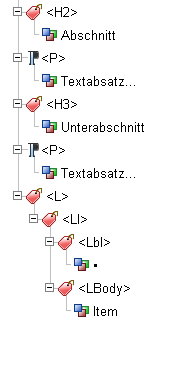
\includegraphics[width=1\textwidth]{images/flatstructure}
%		\end{minipage}
%		\hfill
%		\begin{minipage}[t]{0.30\columnwidth}%
%		\minisec{Struktur mit \optname{highstructure}}\vspace{\lineheight}
%			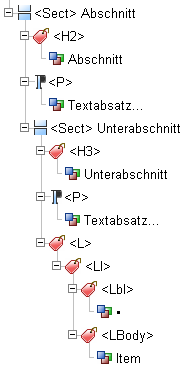
\includegraphics[width=1\textwidth]{images/highstructure}
%		\end{minipage}
%	\caption{Erläuterungen zu flachen und strukturierten Variante}
%	\label{fig:highflatstructure}
%\end{figure}
%
%Unter Verwendung der Option \optname{highstructure} wird eine durch \pdfname{Sect}-Elemente tiefer verschachtelte Struktur erzeugt. Gerade in größeren, gut strukturierten Latex-Dokumenten enthält der Baum auf der ersten Ebene nur die \pdfname{Sect}-Objekte der Kapitel oder Teile (Parts), je nachdem welche die höchste Ebene der Dokumentenklasse ist. Für längere Dokumente ist diese Variante übersichtlicher. Für kürzere Dokumente hingegen ist die flache Strukturierung durchaus ausreichend.
%
%\section{Die Befehle}
% %%%%%%%%%%%%%%%%%%%%%%%%
%Für den normalen Autor führt das Paket \packname{accessibility} nur wenige neue Befehle ein. Es erzeugt die Struktur vielmehr durch bestmögliches transparentes Umdefinieren der Standard-Latex-Befehle. Diese können größtenteils wie gewohnt verwendet werden. Eine ausführliche Anleitung finden Sie in der zugehörigen Autorenanleitung \cite{schalitz07}.
%
%Neue Befehle dienen der Erhöhung der Accessibility im Ergebnisdokument, also dem PDF. Für Grafiken und Formeln steht nun ein Befehl \comname{alt} für alternative Beschreibungen bereit. Er muss nach Möglichkeit am Anfang der Umgebung stehen und sollte reinen ASCII-Text enthalten. Die Zeichen "`|^, {, }, [, ],_|"' können verwendet werden, auf die Verwendung des "`|\|"' ist hingegen zu verzichten. Eine mögliche Verwendung zeigt die Abbildung	\ref{fig:verwendungalt}.
%
%\begin{figure}[htbp]
%		\hfill
%		\begin{minipage}[t]{0.40\columnwidth}%
%		\minisec{Einbinden einer Grafik}\vspace{\lineheight}
%		\begin{verbatim}
%		\begin{figure}[htbp]
%		  \alt{Hier die alternative
%		   Beschreibung der Figure angeben.}
%		  \includegraphics{beispielbild}
%		  \caption{Beispielbild}
%		\end{figure}
%		\end{verbatim}
%		\end{minipage}
%		\hfill
%		\begin{minipage}[t]{0.40\columnwidth}%
%		\minisec{Einbindung einer Formel}\vspace{\lineheight}
%		\begin{verbatim}
%		\begin{equation}
%		  \alt{c = sqrt{a^{2}+b^{2}}}
%		  c = \sqrt{ a^{2}+b^{2} }
%		\end{equation}
%		\end{verbatim}
%		\end{minipage}
%		\hfill
%	\caption{Beispiel für die Verwendung alternativen Beschreibungen}
%	\label{fig:verwendungalt}
%\end{figure}
%
%Des Weiteren ist insbesondere bei der Beschreibung von Formeln von der Wiedergaben von Layoutbefehlen (wie fett, kursiv oder Ausrichtungsbefehle) abzuraten. Es sollte auf eine sinnvolle Strukturierung der Beschreibung mittels Leerzeichen und eindeutige Klammerung geachtet werden.
%
%\StopEventually{%
%	\bibliographystyle{geralpha}
%	\bibliography{references}
%}%
% %%%%%%%%%%%%%%%%%%%%%%%%%%%%%%%%%%%%%%%%%%%%%%%%%%%%%%%%%%%%%%%%%%%
%\chapter{Die Implementierung}
% %%%%%%%%%%%%%%%%%%%%%%%%
%
%Die Implementierung basiert auf der Manipulation des PDF-Outputs über die Schnittstelle von \packname{pdftex}. Dabei werden insbesondere die Befehle \comname{pdfliteral} und \comname{pdfobj} genutzt. Diese Primitiven fügen den übergebenen Text direkt in den Quellcode der PDF-Datei ein. Er muss der zugrunde liegenden Spezifikation folglich entsprechen. Ansonsten wird ein nicht valides Dokument erzeugt.
%
%Für detailliertere Ausführungen, wie und warum das Paket \packname{accessibility} entstand, ist die Diplomarbeit "`Erhöhung von Accessibility in \LaTeX-Dokumenten"' \cite{schalitz2007} zu konsultieren. Sie enthält ein umfassendes Konzept sowie tiefer gehende Erläuterungen zum PDF.
%
%\section{Der Vorspann}
% %%%%%%%%%%%%%%%%%%%%%%%%
%
%\subsection{Paketinformationen und benötigte Pakete}
% %%%%%%%%%%%%%%%%%%%%%%%%
%
%Dieses Paket sollte mit allen \LaTeXe\ Versionen zusammenarbeiten, wurde aber nur mit der Version vom 1. Juni 2000 getestet.
% ^^A VERSION INFO 3 OF 3
%
%    \begin{macrocode}
%<*package>
\ProvidesPackage{accessibility}[2019/11/02 v. 2.0.3]
\NeedsTeXFormat{LaTeX2e}
%    \end{macrocode}

%
%Zunächst werden einige benötigte Pakete geladen.
%
%    \begin{macrocode}
\RequirePackage{xkeyval}
\RequirePackage{ifthen}
%    \end{macrocode}

%
%\subsection{Variablendeklaration}
% %%%%%%%%%%%%%%%%%%%%%%%%
%
%Die Variablen werden benötigt, um später den Strukturbaum aufzubauen. Für die Objektnummern der PDF-Objekte wird jeweils ein Zähler gebraucht.
%
%Das Wurzelelement (\pdfname{StructTreeRoot}) wird in Zähler \varname{StructTree} gehalten. Dazu wird ein neues PDF-Objekt reserviert und die Nummer zur späteren Verwendung gespeichert. Das \varname{Karray} dient der Speicherung sämtlicher Objektreferenzen, die dem Wurzelobjekt untergeordnet werden. Es ist anfangs leer.
%    \begin{macrocode}
\newcounter{StructTree}%
\pdfobj reserveobjnum%
\setcounter{StructTree}{\pdflastobj}%
\xdef\Karray{}%
%    \end{macrocode}

% Zur kurzzeitigen Zwischenspeicherung von Objektnummern steht der Zähler \varname{ObjHelp} zur Verfügung.
%    \begin{macrocode}
\newcounter{ObjHelp}%
%    \end{macrocode}

%Der Zähler \varname{TaggedObj} hält die aktuelle \pdfname{MCID} des ausgezeichneten Objektes, um die Verbindung zum Strukturbaum herzustellen. Laut PDF-Referenz wird diese ID für jedes Seitenobjekt zurückgesetzt. Da der Seitenzähler aber erst nach |\shipout| berichtigt wird, stimmt die Seitenreferenz für die bis dahin geschrieben Objekte nicht. Es kommt zu doppelten ID auf einer Seite, was die eindeutige Zuordnung stört und zahlreiche Fehler birgt. Folgefehler dieses Problems künnen durch die durchgehenden Nummerierung beseitigt werden.
%    \begin{macrocode}
\newcounter{TaggedObj}%[page]
%    \end{macrocode}

%In dem Schalter \varname{ACCESSProblems} wird gespeichert, ob noch Bedenken bezüglich der Accessibility des Dokumentes bestehen, also z.~B. alternative Texte nicht gesetzt wurden oder ähnliches.
%    \begin{macrocode}
\newboolean{ACCESSProblems} \setboolean{ACCESSProblems}{false}%
%    \end{macrocode}
%
%Diese Variablen dienen der Speicherung der aktuellen Sprache sowie der Unterscheidung, ob die Sprache geändert wurde.
%    \begin{macrocode}
\gdef\DocumentLanguage{}%
\gdef\ActualLanguage{}%
\newif\ifLanguageDiff \global\LanguageDifffalse%
\gdef\LanguageCode{}%
%    \end{macrocode}
%
%\varname{DetailedStructure} dient der Feststellung, ob eine geschachtelte oder flache Struktur erzeugt werden soll. Während \varname{@Access@pdf} wahr ist, wenn Tagged PDF erzeugt werden soll und eine geeignete \packname{pdftex}-Version aktiv ist.
%    \begin{macrocode}
\newboolean{@tagged@pdf} \setboolean{@tagged@pdf}{false}%
\newboolean{@right@pdfversion} \setboolean{@tagged@pdf}{false}%
\newboolean{@Access@pdf} \setboolean{@Access@pdf}{false}%
\newif\ifPDFDetailedStructure \global\PDFDetailedStructuretrue%
%    \end{macrocode}
%
%\subsection{Definition der Optionen}
% %%%%%%%%%%%%%%%%%%%%%%%%
%Hier werden die möglichen Optionen deklariert und passende Variablen für die Weiternutzung initialisiert.
%    \begin{macrocode}
\DeclareOption{flatstructure}{\global\PDFDetailedStructurefalse}%
\DeclareOption{highstructure}{\global\PDFDetailedStructuretrue}%
\DeclareOption{tagged}{\setboolean{@tagged@pdf}{true}}%
\DeclareOption{untagged}{\setboolean{@tagged@pdf}{false}}%
\DeclareOption*{%
   \PackageWarning{accessibility}{Unknown Option \CurrentOption}}%
\ProcessOptions\relax%
%    \end{macrocode}

%
%\subsection{Überprüfen des Ausgabemodus}
% %%%%%%%%%%%%%%%%%%%%%%%%
%
%An dieser Stelle wird der Ausgabemodus sowie die verwandte PDFTEX-Version getestet, erst ab der Version 1.20 kann direkter PDF-Output generiert werden.

%    \begin{macrocode}
\ifthenelse{\isundefined{\pdfoutput}}{%
  %latex with dvips
  \setboolean{@right@pdfversion}{false}%
  }{\ifthenelse{\number\pdfoutput<1}{%
      %pdflatex in DVI mode
      \setboolean{@right@pdfversion}{false}%
      }{%pdflatex in PDF mode
      \ifthenelse{\pdftexversion<120}{%
          \PackageError{accessibility}%
          {pdfTeX/pdfLaTeX version >= 1.20 required for direct PDF outut}%
          {Try to install a more recent version!}%
      }{%
      %It is the right version
      \setboolean{@right@pdfversion}{true}%
    }%
  }%
}
%    \end{macrocode}

%Nur wenn beide Bedingungen erfüllt sind, wird im weiteren Verlauf "`Tagged"' PDF erzeugt.
%    \begin{macrocode}
\ifthenelse{\boolean{@right@pdfversion} \and \boolean{@tagged@pdf}}{%
      \setboolean{@Access@pdf}{true}%
}{%
      \setboolean{@Access@pdf}{false}%
}
%    \end{macrocode}

%
%\subsection{Überprüfen der Dokumentenklasse}
% %%%%%%%%%%%%%%%%%%%%%%%%
%
%Da die bereitgestellten logischen Befehle je nach gewählter Dokumentenklasse variieren, wird hier zwischen den Standardklassen und denen des Koma-Scripts unterschieden.
%    \begin{macrocode}
\newboolean{@KOMAScriptClass} \setboolean{@KOMAScriptClass}{false}%

\@ifclassloaded{scrreprt} {\setboolean{@KOMAScriptClass}{true}}{}%
\@ifclassloaded{scrbook}  {\setboolean{@KOMAScriptClass}{true}}{}%
\@ifclassloaded{scrartcl} {\setboolean{@KOMAScriptClass}{true}}{}%
\ifthenelse{\boolean{@KOMAScriptClass}}{%
                \PackageInfo{accessibility}{KOMAscript Klasse}}{}%

\newboolean{@StandardClass} \setboolean{@StandardClass}{false}%

\@ifclassloaded{report} {\setboolean{@StandardClass}{true}}{}%
\@ifclassloaded{book}   {\setboolean{@StandardClass}{true}}{}%
\@ifclassloaded{article}{\setboolean{@StandardClass}{true}}{}%

\ifthenelse{\boolean{@StandardClass}}{%
               \PackageInfo{accessibility}{Standardklasse}}{}%
%    \end{macrocode}

%Noch einige sinnvolle Variablenbelegungen zur PDF-Erzeugung. Sie müssen im fertigen Code nicht mehr enthalten sein.
%    \begin{macrocode}
\pdfcompresslevel=0% Damit wird die PDF-Quelldatei lesbar
\pdfminorversion=6% Bestimmt die PDF - Version der Ausgabe
%\pdfadjustspacing=0% 0, 1 oder 2 änderung nicht erkannt
%    \end{macrocode}

%\subsection{Definition der neuen Befehle}
% %%%%%%%%%%%%%%%%%%%%%%%%
%An dieser Stelle werden die neu eingeführten Befehle für die benötigten Zusatzinformationen definiert.
%    \begin{macrocode}
\newcommand{\alt}[1]{\xdef\altAttr{#1}}%
\newcommand{\newhref}[3]{\xdef\altAttr{#2}\href{#1}{#3}}%
  %
\@ifundefined{thead}{%
  \newcommand{\thead}[1]{%
    \global\TableHeadCelltrue%
    \textbf{#1}}%
}{%
  \let\originalthead\thead
  \renewcommand{\thead}{%
    \global\TableHeadCelltrue%
    \originalthead}%
}
%    \end{macrocode}

%
%\section{allgemeine Hilfsmakros}
% %%%%%%%%%%%%%%%%%%%%%%%%
%
%\subsection{Der Stack}
% %%%%%%%%%%%%%%%%%%%%%%%%
%Der Strukturbaum, lässt sich am einfachsten über einen Stack aufbauen. Prinzipiell müssen für alle Strukturelemente drei Variablen initialisiert werden, nämlich der Strukturtyp, die Objektnummer und das Feld mit den Kindelementen. Für einige Elemente macht Sinn einen Titel zu generieren bzw. zu übergeben, damit wird der generische Strukturtyp näher spezifiziert.
%
%Diese Informationen werden sowohl benötigt, um Kindelemente zu erzeugen. Als auch bei der Beendigung, also dem eigentlichen Schreiben des Strukturobjektes. Ein Zugriff ist dabei immer nur auf das oberste Element möglich. Es muss beendet werden, bevor ein darrunterliegendes abgeschlossen werden kann. Für die effektive Arbeit mit dem Stack werden 3 Funktionen benötigt.
%
%\begin{macro}{\accessPushStack}
%Zum einen benötigt man eine Funktion um Elemente auf dem Stack abzulegen.
%\paragraph{Parameter}
%|#1| Type |#2| ObjNum |#3| KidsField |#4| Title
%    \begin{macrocode}
\newcount\@stackdepth \@stackdepth=0%
\def\accessPushStack#1#2#3#4{%
   \ifnum \@stackdepth >15\relax%
        \PackageWarning{accessibility}{too deep}%
   \else%
        \global\advance\@stackdepth\@ne%
   \fi%
    {\expandafter\xdef\csname StackA\romannumeral\the\@stackdepth\endcsname{#1}}%
   {\expandafter\xdef\csname StackB\romannumeral\the\@stackdepth\endcsname{#2}}%
   {\expandafter\xdef\csname StackC\romannumeral\the\@stackdepth\endcsname{#3}}%
   {\expandafter\xdef\csname StackD\romannumeral\the\@stackdepth\endcsname{#4}}%
}%
%    \end{macrocode}

%\end{macro}
%
%\begin{macro}{\accessPopStack}
%Des Weiteren ist es nötig Elemente vom Stack zu entfernen und abzuarbeiten.
%\paragraph{Parameter}
%|#1| Type |#2| ObjNum |#3| KidsField |#4| Title
%    \begin{macrocode}
\def\accessPopStack#1#2#3#4{%
  \ifnum \the\@stackdepth <1\relax%
     \global\let#1\empty%
     \global\let#2\empty%
     \global\let#3\empty%
     \global\let#4\empty%
  \else%
     \xdef#1{\csname StackA\romannumeral\the\@stackdepth\endcsname}%
     \xdef#2{\csname StackB\romannumeral\the\@stackdepth\endcsname}%
     \xdef#3{\csname StackC\romannumeral\the\@stackdepth\endcsname}%
     \xdef#4{\csname StackD\romannumeral\the\@stackdepth\endcsname}%
   %Variablen wieder leeren
   {\expandafter\xdef\csname StackA\romannumeral\the\@stackdepth\endcsname{}}%
   {\expandafter\xdef\csname StackB\romannumeral\the\@stackdepth\endcsname{}}%
   {\expandafter\xdef\csname StackC\romannumeral\the\@stackdepth\endcsname{}}%
   {\expandafter\xdef\csname StackD\romannumeral\the\@stackdepth\endcsname{}}%
     \global\advance\@stackdepth\m@ne%
  \fi%
}%
%    \end{macrocode}

%\end{macro}
%
%\begin{macro}{\accessReadTopStack}
%Zum anderen wird wären der Erzeugung von Blattknoten ein lesender Zugriff auf das oberste Stackelement benötigt. Somit kann die Objektreferenz in dass Kinderfeld des Elternelementes eingetragen werden und eine Referenzierung des Elternobjektes wird möglich.
%\paragraph{Parameter}
%|#1| Type |#2| ObjNum |#3| KidsField
%    \begin{macrocode}
\def\accessReadTopStack#1#2#3{%
  \ifnum \the\@stackdepth <1\relax%
     \global\let#1\empty%
     \global\let#2\empty%
     \global\let#3\empty%
  \else%
     \xdef#1{\csname StackA\romannumeral\the\@stackdepth\endcsname}%
     \xdef#2{\csname StackB\romannumeral\the\@stackdepth\endcsname}%
     \xdef#3{\csname StackC\romannumeral\the\@stackdepth\endcsname}%
  \fi%
}%
%    \end{macrocode}

%\end{macro}

%Die folgenden Makros schreiben die tatsächlichen Elemente in die PDF-Datei, zur flexiblen Nutzung sind die übergabeparameter variabel.
%
%\subsection{Reine Strukturelemente}
% %%%%%%%%%%%%%%%%%%%%%%%%
%
%\begin{environment}{PDFStructObj}
%Ein PDFStructObj ist eine Struktur, die dazu dient weitere Elemente zu kapseln. Die benötigten Variablen werden initialisiert und anschließend jeweils auf den Stack geschrieben.
%
%\paragraph{Parameter}
%|#1| StructType |#2| Title
%    \begin{macrocode}
\newenvironment{PDFStructObj}[2]{% #1 StructType #2 Title
  \ifTextActive{\endPDFMarkContent\endPDFTextObj}\fi%
  \pdfobj reserveobjnum% Objektnummer reservieren
  \setcounter{ObjHelp}{\pdflastobj}%
  \expandafter\xdef\csname PDF@#1@Array\endcsname{}%
  \accessPushStack{#1}{\theObjHelp}{PDF@#1@Array}{#2}%drauftun
}%
%    \end{macrocode}
%Zum Abschluss eines PDFStructObj wird das oberste Element vom Stack geholt. Ist dieser leer, was sich darin zeigt, dass das \varname{StructElem} leer ist, wird eine Warnung ausgegeben. Diese Abfrage erhöht die Stabilität, der Fall sollte aber normalerweise nicht auftreten.
%
%Im jedem anderen Fall werden die Attribute geprüft und gesetzt. Anschließend wird das PDF-Objekt erzeugt und eine Referenz in das Elternelement eingefügt.
%
%Die Erzeugung von reinen Strukturobjekten erfolgt ohne Seitenreferenz, da die Unterelemente potentiell auf mehrere Seiten verteilt sein können.
%    \begin{macrocode}
{%andere Ebenen Schließen
  \accessPopStack\StructElem\Objnum\KidsArray\Title		%runterholen
  \ifx \StructElem\empty%
    \PackageWarning{accessibility}{empty \string\PopStack ?}%
  \else%
    %\convertLanguageInCode{\languagename}%
    \gdef\TitleHelp{}%
    \if \Title\empty \else%
        \gdef\TitleHelp{/T (\Title)}%
    \fi%
     \ifnum \@stackdepth <1\relax%
          \xdef\ParentElem{\theStructTree}%
          \xdef\ParentArray{Karray}%
     \else%
          \accessReadTopStack\ParentStructElem\ParentElem\ParentArray%
     \fi%
    \immediate \pdfobj useobjnum\number\Objnum{<</Type /StructElem %
        /P \ParentElem\space 0 R %
        \TitleHelp %
        /C /Normal %
        \space\LanguageCode %
        /K [\csname \KidsArray\endcsname] %
        /S /\StructElem>>}%
    \pdfrefobj\Objnum%
    \expandafter\xdef\csname \ParentArray\endcsname{%
         \csname \ParentArray\endcsname \space \Objnum\space 0 R}%
  \fi%
}
%    \end{macrocode}

%\end{environment}
%\begin{TODO}Für Blockelemente keine Sprache, tlw. zu spät geschossen $\rightarrow$ Probleme bei Sprachauszeichnung. \end{TODO}
%
%\subsubsection{Implizite Beendigung von Strukturelemente}
% %%%%%%%%%%%%%%%%%%%%%%%%
%
%In \LaTeX\ werden viele Strukturen nur begonnen aber nicht explizit wieder geschlossen. Z.~B. schließt eine \comname{section} die geöffnete \comname{subsection} indem sie die Zähler zurücksetzt. Es existiert folglich auch in \LaTeX\ eine wohl definierte Hierarchie.
%
%\begin{macro}{\sectionInDepth}
%Ordnet den Strukturelementen eine Reihenfolge zu, damit diese in der richtigen Reihenfolge automatisch geschlossen werden können.
%    \begin{macrocode}
\newcommand{\sectionInDepth}[2]{%
   \csname #2\endcsname=100%
   \ifthenelse{\equal{#1}{Document}}{\csname #2\endcsname=\m@ne}{}%
   \ifthenelse{\equal{#1}{Part}}{\csname #2\endcsname=0}{}%
   \ifthenelse{\equal{#1}{Chapter}}{\csname #2\endcsname=1}{}%
   \ifthenelse{\equal{#1}{Section}}{\csname #2\endcsname=2}{}%
   \ifthenelse{\equal{#1}{Subsection}}{\csname #2\endcsname=3}{}%
   \ifthenelse{\equal{#1}{Subsubsection}}{\csname #2\endcsname=4}{}%
   \ifthenelse{\equal{#1}{Paragraph}}{\csname #2\endcsname=5}{}%
   \ifthenelse{\equal{#1}{Subparagraph}}{\csname #2\endcsname=6}{}%
   \ifthenelse{\equal{#1}{Div}}{\csname #2\endcsname=7}{}%
}
%    \end{macrocode}

%\end{macro}
%

%
%\begin{macro}{\closeUntilPDFStruct}
%Schließt die Sectionebenen unter Verwendung der eben definierten Reihenfolge automatisch. Damit wird die Schachtelung wesentlich flexibilisiert. Es gibt keine Fehler wenn eine Ebene fehlt.
%
%Einige Variablen die im Macro benötigt werden.
%    \begin{macrocode}
\newcount\@bool%
\newcount\@elem%
\newcount\@elemi%
%    \end{macrocode}
%
%Zu allererst muss eventuell noch offener Text beendet werden. Anschließend beendet eine Schleife solange das jeweils oben aufliegende Stackelement, bis die nötige Tiefe erreicht ist. Ein Kapitel beendet alle Strukturen höherer Nummer, aber maximal ein Kapitel.
%    \begin{macrocode}
\newcommand{\closeUntilPDFStruct}[1]{%
      \ifTextActive%
          \endPDFMarkContent%
          \endPDFTextObj%
      \fi%
     %Schleife
     \@bool=0%
        \sectionInDepth{#1}{@elemi}%
        \ifnum \@elemi=100 \@bool=1 \fi%
        \global\advance\@elemi\m@ne%
     \@whilenum \@bool =0\do{%
        \accessReadTopStack\StructElem\Objnum\KidsArray%
        \sectionInDepth{\StructElem}{@elem}%
        \ifthenelse{\@elem >\@elemi}{%
             \endPDFStructObj%
        }{%
             \@bool=1%
        }%
        \if #1\empty \@bool=1 \fi%
        \ifthenelse{\equal{#1}{\StructElem}}{\@bool=1}{}%
     }%
}
%    \end{macrocode}

%\end{macro}
%
%\subsection{Normale und besondere Textelemente}
% %%%%%%%%%%%%%%%%%%%%%%%%
%
%Sie enthalten Textabsätze und eventuell weitere Objekte auf Zeilenebene wie Fußnoten, Referenzen, Formeln, Zitat.... Ein spezielles Textelement (wie Zitat, Formel, Quellcode...) wird durch Befehle oder Umgebungen gesondert hervorgehoben. Normale Textelemente sind hingegen nicht markiert. Eine Erkennung wird durch \comname{everypar} erzielt. Diese Funktion wird zu Beginn jedes neuen Textabschnittes im vertikalen Modus verwendet.
%
%Es ist immer maximal ein Textobjekt aktiv. Textobjekte können nicht ineinander geschachtelt werden.
%
%\begin{environment}{PDFTextObj}
%Ist eine Strukturobjekt, dass normale Textpassagen auf Absatzebene enthält.
%
% Einige Variablen die für die folgende Definition benötigt werden.
%    \begin{macrocode}
\xdef\TextType{}%
\newcounter{TextObjNum}%
\xdef\TextArray{}%
\newif\ifTextActive \TextActivefalse%
\newif\ifSpezialTextActive \SpezialTextActivefalse%
%    \end{macrocode}

%Zu Beginn eines Textobjektes werden noch offene Textobjekte abgeschlossen. Anschließend werden die benötigten Variablen neu initialisiert.
%    \begin{macrocode}
\newenvironment*{PDFTextObj}{%
  %altes Textobj beenden, immer max. ein Textobj aktiv
  \ifTextActive \endPDFMarkContent\endPDFTextObj\fi%
  %neues anfangen
  \global\TextActivetrue%
  \pdfobj reserveobjnum% Objektnummer reservieren
  \setcounter{TextObjNum}{\pdflastobj}%
  \xdef\TextArray{}%
  \xdef\TextType{P}% kein TextTxp --> P
}%
%    \end{macrocode}
% Um ein Textobjekt abzuschließen wird zunächst das Elternelement ermittelt. Dies liegt normalerweise oben auf dem Stack. Ist dieser leer wird das Element direkt unter der Wurzel eingefügt.
%    \begin{macrocode}
{%
 \ifTextActive%
  \ifnum \@stackdepth <1\relax%
       \xdef\ParentElem{\theStructTree}%
       \xdef\ParentArray{Karray}%
       %\PackageWarning{accessibility}{stackdepth<1}%
  \else%
       \accessReadTopStack\ParentStructElem\ParentElem\ParentArray%
  \fi%
  %\convertLanguageInCode{\languagename}%
  \immediate \pdfobj useobjnum\theTextObjNum{<</Type /StructElem %
     /P \ParentElem \space 0 R %
     /C /Normal %
     /K [\TextArray] %
     /S /\TextType %
    \space\LanguageCode>>}%
  \pdfrefobj \theTextObjNum%
  \expandafter\xdef\csname \ParentArray\endcsname{%
       \csname \ParentArray\endcsname \space \theTextObjNum\space 0 R}%
  \global\TextActivefalse%
 \fi%
}
%    \end{macrocode}

%\end{environment}

%\begin{environment}{PDFSpezialTextObj}
%
%Im Unterschied zu normales Textobjekten sind besondere Textelemente im \LaTeX-Code speziell ausgezeichnet. Eine Erkennung ist also gewissermaßen zuverlässiger möglich. Da es sich bei speziellen Textobjekten auch um z.~B. Formeln handeln kann, werden noch Variablen zur Attributverwaltung eingeführt werden.
%    \begin{macrocode}
\xdef\altAttr{}%
\xdef\titleAttr{}%
%    \end{macrocode}
%
%Der Beginn eines speziellen Textobjektes ist analog dem eines Normalen.
%\paragraph{Parameter}
%|#1| StructType
%    \begin{macrocode}
\newenvironment*{PDFSpezialTextObj}[1]{%
  \ifTextActive \endPDFMarkContent\endPDFTextObj\fi%
  %neues anfangen
  \global\SpezialTextActivetrue%
  \pdfobj reserveobjnum% Objektnummer reservieren
  \setcounter{TextObjNum}{\pdflastobj}%
  \xdef\TextArray{}%
  \xdef\TextType{#1}%
}%
%    \end{macrocode}
%
%Auch das Ende ist bis auf die Verwaltung der Attribute ähnlich. Eine Unterscheidung ist jedoch für spätere Zwecke nötig.
%    \begin{macrocode}
{%
  %\gdef\LanguageHelp{}%
  %\ifLanguageDiff%
  %    \gdef\LanguageHelp{\LanguageCode}%
  %\fi%
  %  \convertLanguageInCode{\languagename}%
    \gdef\AltHelp{}%
  \ifthenelse{\equal{\altAttr}{}}{}{%
     \gdef\AltHelp{/Alt(\altAttr)}%
  }%
  \gdef\TitleHelp{}%
  \ifthenelse{\equal{\titleAttr}{}}{}{%
     \gdef\TitleHelp{/T(\titleAttr)}%
  }%
  \ifnum \@stackdepth <1\relax%
       \xdef\ParentElem{\theStructTree}%
       \xdef\ParentArray{Karray}%
  \else%
       \accessReadTopStack\ParentStructElem\ParentElem\ParentArray%
  \fi%
  \immediate \pdfobj useobjnum\theTextObjNum{<</Type /StructElem %
     /P \ParentElem \space 0 R %
     /C /Normal %
     /K [\TextArray] %
     /S /\TextType %
    \space\LanguageCode %
    \space\TitleHelp %
    \space\AltHelp>>}%
  \pdfrefobj \theTextObjNum%
  \expandafter\xdef\csname \ParentArray\endcsname{%
      \csname \ParentArray\endcsname \space \theTextObjNum\space 0 R}%
  \global\SpezialTextActivefalse%
  \xdef\TextType{}%
  \EveryparReset%
  \xdef\altAttr{}% wieder leeren
  \xdef\titleAttr{}% wieder leeren
}
%    \end{macrocode}

%\end{environment}
%
%\subsection{Elemente auf Zeilenebene}
% %%%%%%%%%%%%%%%%%%%%%%%%
%
%\begin{environment}{PDFInlineObjInText}
%Treten Objekte auf Zeilenebene in Textfluss auf, so muss dieser unterbrochen werden, dass Objekt geschrieben werden und anschließend ist der Textfluss fortzusetzen. Zu diesem Zweck müssen einige Zustandvariablen gespeichert werden.
%
%    \begin{macrocode}
\xdef\lastEveryparType{}%
\xdef\HelpBool{}%
\xdef\Type{}%
\newcounter{PDFReferenceObjNum}%
\xdef\ReferenceArray{}%
%    \end{macrocode}
%Zuerst werden die alten Variablen gesichert. Anschließend ist für den Fall, dass es sich um Referenzen handelt, eine Sonderbehandlung nötig. Ihnen ist zusätzlich das von \packname{hyperref} erzeugte Linkobjekt zu zuordnen. Da im Textfluss \comname{everypar} nicht greift, muss die Markierung des ContentStreams manuell vorgenommen werden.
%    \begin{macrocode}
\newenvironment*{PDFInlineObjInText}[1]{%
  %alte einstellung merken
  \xdef\lastEveryparType{\everyparStructElem}%
  \xdef\HelpBool{\InlineObj}%
  \xdef\Type{#1}%
  \ifthenelse{\equal{\Type}{Reference} \or \equal{\Type}{Link}}{%
    \pdfobj reserveobjnum%
    \setcounter{PDFReferenceObjNum}{\pdflastobj}%
     \setcounter{ObjNum}{\theTaggedObj}%
     \EveryparConfig{#1}{obj}%
  }{%
     \EveryparConfig{#1}{true}%
  }%
  \PDFMarkContent% kein everypar
}%
%    \end{macrocode}
%Anschließend ist die Markierung wieder zu beenden. Für Referenzen und Links muss nun die OBJR mit in die Struktur eingebunden werden. Das funktioniert über pdflastlink, aber erst ab PDFTEX Version 1.4.. Zum Schluss wird der Ausgangszustand wiederhergestellt und der nachfolgende Textfluss markiert.
%    \begin{macrocode}
{%
  \endPDFMarkContent%
  \ifthenelse{\equal{\Type}{Reference} \or \equal{\Type}{Link}}{%
    \xdef\ReferenceArray{<</Type /MCR /Pg \pdfpageref\thepage %
         \space \space 0 R /MCID \theObjNum>>}%
    \ifthenelse{\pdftexversion>139}{%
      \setcounter{ObjHelp}{\pdflastlink}%%<</Type /OBJR /Obj 600 0 R>>
      %\PackageWarning{accessibility}%
      %{Objektnummer vom letzten Link: \theObjHelp}%
      \ifthenelse{\theObjHelp>0}{%
        \xdef\ReferenceArray{\ReferenceArray\space %
              <</Type /OBJR /Obj \theObjHelp\space 0 R>>}%
      }{}%
   }{}%
   \writeComplexTextObj{\thePDFReferenceObjNum}%
         {\ReferenceArray}%
         {/Reference}{\theTextObjNum}{NoPage}%
   \xdef\TextArray{\TextArray \theObjHelp\space 0 R \space}%
  }{}%
  % alte einstellung wiederherstellen
  \EveryparConfig{\lastEveryparType}{\HelpBool}%
  \PDFMarkContent%
}
%    \end{macrocode}

%\end{environment}
%
%
%\subsection{Marked Content}
% %%%%%%%%%%%%%%%%%%%%%%%%
%
%Zusätzlich zum Schreiben der Objekte müssen die zugehörigen Textpassagen im ContentStream markiert werden. Diese Funktionalität deckt das Makro PDFMarkContent ab.
%
%Die Hilfsmakros \comname{EveryparConfig} und \comname{EyeryparReset} dienen der Flexibilisierung von MarkContent, indem sie dort verwendete Variablen setzen. MarkContent ist die Funktion die durch \comname{everypar} aufgerufen wird.

%\begin{macro}{\EveryparConfig}
%Setzt die Variablen auf die übergebenen Werte
%\paragraph{Parameter}
%|#1| EveryparStructElem |#2| true/false/obj
%    \begin{macrocode}
\newcommand{\EveryparConfig}[2]{%
   \xdef\everyparStructElem{#1}%
   \xdef\InlineObj{#2}%
}
%    \end{macrocode}

%\end{macro}
%
%\begin{macro}{\EveryparReset}
%%Setzt die Variablen auf die Standardwerte für eine normale Texterkennung.
%    \begin{macrocode}
\newcommand{\EveryparReset}{%
   \xdef\everyparStructElem{P}%
   \xdef\InlineObj{false}%
}
%    \end{macrocode}

%\end{macro}
%
%\begin{environment}{PDFMarkContent}
%Zunächst werden wieder einige Variablen benötigt. Zum einen muss eine Markierung immer erst beendet werden, bevor eine neue angefangen wird. Der Sicherung dient die Variable \varname{MarkContentOpen}. Auch die Markierung enthält einen Typ, der im allgemeinem denen des Textobjektes entspricht.
%
%Die erzeugten Markierungen werden anschließend dem Strukturbaum zugeordnet. Dabei ist eine direkt Einbindung als MarkContentReferenz möglich, oder es kann ein Blattknoten erzeugt werden, der die Verbindung herstellt. Die Unterscheidung wird mittels \varname{InlineObj} vorgenommen. Sie kann bisher die Belegungen {true, false und obj} annehmen.
%    \begin{macrocode}
\newif\ifMarkContentOpen \MarkContentOpenfalse%
\xdef\everyparStructElem{P}%
\xdef\InlineObj{false}%
%    \end{macrocode}
%
%Zunächst wird eine eventuell geöffnete Markierung abgeschossen. Anschließend wird eine neue Markierung unter Verwendung der Funktion \comname{pdfliteral} in den ContentStream eingefügt. Da der Anfang einer nötigen Markierung zuverlässiger zu Erkennen ist, als das Ende wird die Verbindung zum Strukturbaum gleich anschließend durchgeführt. Des Weiteren werden Schachtelungsprobleme vermieden, bei denen die Zuordnung der MCID durch überschreibung des \varname{TaggedObj} ungültig wird.
%    \begin{macrocode}
\newenvironment{PDFMarkContent}{%
  \ifMarkContentOpen \endPDFMarkContent\fi%
  \global\MarkContentOpentrue%
  \ifthenelse{\equal{\everyparStructElem}{}}{\EveryparReset}{}%
  \pdfliteral{/\everyparStructElem\space <</MCID \theTaggedObj>> BDC}%
  \ifthenelse{\equal{\InlineObj}{false}}{% Text
    %\ifthenelse{\equal{\themypage}{\thepage}}{}{%
       %\PackageWarning{accessibility}{unterschiedlich %
       %\thepage<>\themypage; MCID \theTaggedObj}
    %}%
    \xdef\TextArray{\TextArray \space <</Type /MCR %
        %/Pg \pdfpageref\thepage \space \space 0 R %
        /Pg \pdfpageref\themypage \space \space 0 R %
        /MCID \theTaggedObj>>}%
  }{}%
  \ifthenelse{\equal{\InlineObj}{true}}{%  inline-Objekt
    \writePDFLeafObj{\theTaggedObj}{\everyparStructElem}%
  }{}%
  \stepcounter{TaggedObj}%
}%
%    \end{macrocode}
%Wie bereits gesagt, sind die Enden von Absätzen nicht wirklich zuverlässig erkennbar, so dass häufig erst bei dem Beginn einer neuen Struktur auf ein Ende geschlossen werden kann. Eine frühest mögliche Erkennung ist insbesondere an Stellen des Seitenumbruchs relevant. Das Ende soll nach Möglichkeit noch auf der alten Seite auftauchen und nicht erst mit Beginn der neuen Struktur am Beginn der neuen Seite. Eine Verwendung von \comname{endMarkContent} ist relativ bedenkenlos mehrfach möglich, dafür dass nicht zu oft beendet wird, sorgt die Abfrage.
%    \begin{macrocode}
{%
 \ifMarkContentOpen%
    \pdfliteral{EMC}%
    \global\MarkContentOpenfalse%
 \fi%
}
%    \end{macrocode}

%\end{environment}
%
%Zur besseren übersichtlichkeit und wurde das Makro \comname{writePDfLeafObj} ausgelagert. Es kann so des Weiteren auch an anderer Stele wiederverwendet werden.
%
%\begin{macro}{\writePDFLeafObj}
%Diese Makro ermöglicht die Erzeugung einfacher Blattknoten, also derjenigen, die selbst keine Elemente mehr enthalten. Sie referenzieren die \pdfname{MCID} des zugehörigen Textabschnittes, diese wird normalerweise im Zähler \varname{TaggedObj} gehalten, für einige Elemente muss jedoch von dieser Nummerierung abgewichen werden, die Variable in im ersten Argument und der Strukturtyp im zweiten zu übergeben.
%
%\paragraph{Parameter}
%|#1| MCID |#2| Structure
%    \begin{macrocode}
\newcommand*{\writePDFLeafObj}[2]{%
  %\gdef\LanguageHelp{}%
  %\ifLanguageDiff%
  %    \gdef\LanguageHelp{\LanguageCode}%
  %\fi%
  %  \convertLanguageInCode{\languagename}%
  \gdef\AltHelp{}%
  \ifthenelse{\equal{\altAttr}{}}{}{%
     \gdef\AltHelp{/Alt(\altAttr)}%
  }%
  \gdef\TitleHelp{}%
  \ifthenelse{\equal{\titleAttr}{}}{}{%
     \gdef\TitleHelp{/T(\titleAttr)}%
  }%
  \immediate \pdfobj {<</Type /StructElem %
    /P \theTextObjNum \space 0 R %
    /C /Normal %
    /K <</Type /MCR %
         /Pg \pdfpageref\thepage \space \space 0 R %
         /MCID #1>> %
    /S /#2 %
    \space\LanguageCode %
    \space\TitleHelp %
    \space\AltHelp>>}%
  \setcounter{ObjHelp}{\pdflastobj}%
  \pdfrefobj \pdflastobj%
  \xdef\TextArray{\TextArray \space \theObjHelp\space 0 R}%
  \xdef\altAttr{}%
  \xdef\titleAttr{}%
}
%    \end{macrocode}

%\end{macro}

%\begin{macro}{\writeComplexTextObj}
%Komplexere Objekte wie die von Fußnoten, in denen zusätzlich die Strukturen am Seitenende integriert werden, sind mit \comname{writePDFLeafObj} nicht zu realisieren. Diese Funktionalität bietet dieses Makro. Es sind ermöglicht die Erzeugung von mittleren Knoten, also denjenigen, die selbst weitere Objekte enthalten. Damit die doppelte Verlinkung (Eltern mit Kindern, wie umgekehrt) möglich ist, muss bei der Erzeugung der Kinderelemente die Objektnummer des Elternobjektes bekannt sein. Des Weiteren wird jeweils die Referenz des Kindes in die Kinderliste der Eltern eingefügt. So dass dieses erst nach der Generierung aller Kinder erzeugt werden kann. Zur Realisierung wird am Anfang einer mittleren Struktur eine Objektnummer reserviert, die im ersten Parameter übergeben.
%
%Die Erzeugung von Objekten kann sowohl mit, als auch ohne Seitenreferenz erfolgen. Zudem muss die Liste der Kinder, das Elternelement und der Strukturtyp an das Makro übergeben werden.
%
%\paragraph{Parameter}
%|#1| Objektnummer |#2| KidsArray |#3| StructurType |#4| ParentObj |#5| (no)page
%    \begin{macrocode}
\newcommand*{\writeComplexTextObj}[5]{%
  \ifthenelse{\equal{#5}{Page}}{% Seitenreferenz angeben
    \immediate \pdfobj useobjnum#1{<</Type /StructElem %
      /P #4\space 0 R %
      /Pg \pdfpageref\thepage \space \space 0 R %
      /C /Normal %
      /K [#2] %
      /S #3 \space\LanguageCode>>}%
    }{%keine Seitenreferenz angeben
    \immediate \pdfobj useobjnum#1{<</Type /StructElem %
      /P #4\space 0 R %
      /C /Normal %
      /K [#2] %
      /S #3>>}%
  }%
  \setcounter{ObjHelp}{\pdflastobj}%
  \pdfrefobj \pdflastobj%
}
%    \end{macrocode}

%\end{macro}
%
% %%%%%%%%%%%%%%%%%%%%%%%%%%%%%%%%%%%%%%%%%%%%%%%%%%%%%%%%%%%%%%%%%%%
%\section{Erkennen von Absätzen}
% %%%%%%%%%%%%%%%%%%%%%%%%
%
%Da Textabsätze in \LaTeX\ nicht explizit ausgezeichnet sind, wird \comname{everypar} verwendet um den Anfang eines Textabschnittes zu erkennen. Sobald eine andere Struktur erkannt wird, wird der Textabschnitt beendet. In längeren Strukturen wird die Absatzerkennung mit \comname{everypar} explizit ausgesetz und nach Abschluss wieder aktiviert.
%
%\varname{numberingpars} dient der Unterscheidung, ob Absatznummern generiert werden sollen oder eben nicht. Während \varname{npar} von jedem \comname{everypar} zurückgesetzt wird und bestimmt, ob der folgende Absatz nummeriert sein soll. In Kombination ergeben beide ein Werkzeug zur Entscheidung, ob \comname{everypar} nun einen wirklichen Textabsatz einleitet.
%
%Der Zähler \varname{ParCounter} dient nur zu Testzwecken, er zählt die wirklichen Textabsätze je Seite mit. Es ist z.~B. möglich auskommentierten Zeilen zu aktivieren, um z sehen an welchen Stellen \comname{everypar} greift.
%    \begin{macrocode}
  %\newcounter{ParCounter}[page]%
\newcounter{ParCounter}%
\newif\ifnumberingpars \numberingparstrue%
\newif\ifnpar \npartrue%
%    \end{macrocode}

%
%Nun wird die Funktion \comname{everypar} tatsächlich umdefiniert. Dazu werden zunächst die ursprüngliche Definition in \comname{originaleverypar} sowie die Token der Funktion gesichert. Anschließend wird \comname{everypar} unter Verwendung der Originaldefinition erweitert. Ist nun die Textabsatzerkennung bestehend aus \varname{numberingpars} und \varname{npar} aktiviert. Löst \comname{everypar} den Start der Umgebung \comname{PDFText} aus. Sofern diese noch aktiv ist, wird sie zuvor beendet.
%    \begin{macrocode}
\ifthenelse{\boolean{@Access@pdf}}{%
  \let\originaleverypar\everypar%
  \newtoks\npeverypar%
  \npeverypar{}%
  % Call everypar with the argument extended with the toks
  \def\everypar#1{%
    \originaleverypar{#1\ifnumberingpars\the\npeverypar\fi}}%
  \npeverypar{%
    \ifnpar{%
      \stepcounter{ParCounter}%
     %\pdfliteral{/Artifact BMC}%
     % \llap{\small\arabic{ParCounter}\qquad}%
     %\pdfliteral{EMC}%
      \ifSpezialTextActive\else \PDFTextObj \fi%
      \PDFMarkContent%
    }\fi%
  }%
}{}
%    \end{macrocode}
%
% %%%%%%%%%%%%%%%%%%%%%%%%%%%%%%%%%%%%%%%%%%%%%%%%%%%%%%%%%%%%%%%%%%%
%\section{Dokumentbeginn}
% %%%%%%%%%%%%%%%%%%%%%
% Strukturbaum eröffnen.
%    \begin{macrocode}
\AtBeginDocument{%
\PDFStructObj{Document}{\empty}%
\everypar{}%
}
%    \end{macrocode}

% %%%%%%%%%%%%%%%%%%%%%%%%%%%%%%%%%%%%%%%%%%%%%%%%%%%%%%%%%%%%%%%%%%%
%\section{Dokumentende}
% %%%%%%%%%%%%%%%%%%%%%%%%
%Strukturbaum abschließen
%    \begin{macrocode}
\ifthenelse{\boolean{@Access@pdf}}{%
  \AtEndDocument{%
%    \end{macrocode}
%Am Ende des Dokumentes müssen alle noch offenen Strukturen abgeschlossen werden. Diesen Zweck erfüllen die folgenden Zeilen.
%    \begin{macrocode}
  \closeUntilPDFStruct{Document}%
%    \end{macrocode}
%Um in späteren Implementierungen das "`Umfließen"' zu unterstützen muss jedem Strukturelement eine Layout-Klasse zugeordnet werden. Das Klassenzuordnungsobjekt verwaltet diese, in dem es im einfachsten Fall einem Klassennamen (\pdfname{Normal}) verschiedene Layoutattribute zuordnet({\pdfname{TextAlign} \pdfname{Center}). Bisher verhindert die klare Wortbegrenzung (fehlende Leerzeichen) im PDF-Quellcode des ContentStreams ein automatisches Reflow.
%    \begin{macrocode}
  \newcounter{ClassMap}%
  \pdfobj reserveobjnum% neues Objekt Reservieren
  \setcounter{ClassMap}{\pdflastobj}%
  \immediate \pdfobj useobjnum \theClassMap{<<%
      /Normal <</O /Layout /EndIndent 0.0 %
                /SpaceAfter 0.0 /SpaceBefore 0.0 %
                /StartIndent 0.0 /WritingMode %
                /LrTb /TextAlign /Start>> %
      /CM1 <</O /Layout /TextAlign /Justify>> %
      /CM2 <</O /Layout /TextAlign /Center>> %
      /CM3 <</O /Layout /TextAlign /Start>> %
      /CM4 <</O /Layout /InlineAlign /Center %
                /Placement /Block /SpaceAfter 12.125 %
                /BBox [266 314 329 336]>> %
       >>} \pdfrefobj \pdflastobj%
   %\global\setcounter{ClassMap}{\pdflastobj}%
%    \end{macrocode}
%Des Weiteren wurden im Verlauf der Abarbeitung eigene PDF-Strukturen abgeleitet. Sie müssen nun einem Standard-Element zugeordnet werden. Dazu wird das so genannte Rollenzuordnungsobjekt geschrieben. Es ordnet jeweils die selbst definierte (\pdfname{IndexItem}) einer Standardrolle (\pdfname{Span}) zu.
%    \begin{macrocode}
  \pdfobj {<<%
            /IndexItem /Span % Indexeinträge
            /TOF /TOC % Table of Figures
            /TOFI /TOCI % Table of Figures Eintrag
            /TOT /TOC % Table of Tables
            /TOTI /TOCI % Table of Tables Eintrag++
            /Titlepage /Sect % Titlepage
            /Bibliography /L % Bibligraphy
            /BibItem /LI % BibligraphyItem
            /ParagraphSpan /Span % geteilte Paragraphen am Seitenumbruch
            /Footnote /Note %  Fußnotentext
            /Chapter /Sect%
            /Section /Sect%
            /Subsection /Sect%
            /Subsubsection /Sect%
            /Float /Div%
            /L1 /L%
            /L2 /L%
            /L3 /L%
            /L4 /L%
            /L5 /L%
          >>} \pdfrefobj \pdflastobj%
  \setcounter{ObjHelp}{\pdflastobj}%
%    \end{macrocode}
%Erst jetzt, wenn alle Objekte ins PDF-Dokument geschrieben wurden kann, dass Strukturwurzelobjekt erzeugt werden, da es Referenzen auf die anderen Objekte enthält.
%    \begin{macrocode}
  \immediate \pdfobj useobjnum \theStructTree{%
     <</Type /StructTreeRoot %
       /RoleMap \theObjHelp \space 0 R %
       /ClassMap \theClassMap \space 0 R %
       /ParentTree <</Nums [0 [\Karray]]>> % TODO Viel komplizierter
       /ParentTreeNextKey 1 % berechnen
       /K [\Karray] %
     >>}\pdfrefobj\pdflastobj%
%    \end{macrocode}
%Nun wird der gesamte erzeugte Strukturbaum in den Katalog der PDF-Datei eingefügt und das PDF als "`Tagged PDF"' ausgewiesen.
%    \begin{macrocode}
  \pdfcatalog{%
      /StructTreeRoot \theStructTree\space 0 R%
      /MarkInfo <</Marked true /LetterspaceFlags 0>>%
      %/PieceInfo<</MarkedPDF>>%
      %/MarkInfo <</Marked true>>%
      %/Metadata \theStructTree\space 0 R%
      }%
%    \end{macrocode}
%Abschließend wird dem Autor, mitgeteilt, ob und wo noch Probleme bzgl. der Barrierefreiheit bestehen.
%    \begin{macrocode}
  \ifthenelse{\boolean{ACCESSProblems}}{%
     \PackageWarningNoLine{accessibility}{%
        @@@@@@@@@@@@@@@@@@@@@@@@@@@@@@@@@@@@@@@@@@@@@\MessageBreak
        @@ There were non-defined Figure Alt-Tags! @@\MessageBreak
        @@@@@@@@@@@@@@@@@@@@@@@@@@@@@@@@@@@@@@@@@@@@@}%
  }{}%
  }%
}{}
%    \end{macrocode}

%
%\section{Seitenumbruch}
% %%%%%%%%%%%%%%%%%%%%%%%%
%
%Bisher ist eine korrekte Auszeichnung der Seitenumbrüche nicht möglich, da die Autorin bisher keine Variante zur zuverlässigen Erkennung gefunden hat.
%
%Prinzipiell müsste an jedem Seitenende (vor dem Schreiben der Fußnoten) geschaut werden, welche Struktur im ContentStream noch aktiv ist, dass betrifft prinzipiell Elemente wie /P, /Lbody, etc., also Objekte die als Blattobjekte mit einer Seitenreferenz geschrieben werden müssen. Diese müssen durch ein |\pdfliteral{EMC}| unterbrochen werden. Damit wäre immerhin die Integrität des ContentStreams gewährleistest.
%
%\subsection{Automatischer Seitenumbruch}
% %%%%%%%%%%%%%%%%%%%%%%%%
%
%An die richtige Stelle der letzten Seite kann das Literal z.B. mittels |\@textbottom| gesetzt werden. Es wird während der Ausgabe (|\shipout|) aufgerufen. Allerdings gesieht dies nicht genau zum Seitenumbruch, sondern erst nach ein bis zwei Absatzboxen. Damit sind die Variablen wie |ifPDFTextActiv| nicht mehr aktuell und eine Erkennung ist nicht wirklich zuverlässig möglich.
%
%Auf der neuen Seite muss die Struktur dann natürlich wieder geöffnet werden. Dann müssen beide Teile mit der richtigen Seitenreferenz als Element in den Baum einsortiert werden. Beide Funktionen können Inhalte auf der gerade fertiggestellten Seite hinzufügen.
%
%Fußnoten werden im Moment ihres Auftauchens in eine temporäre Box geschrieben und später in den Output eingefügt. |\@texttop| wird immer vor |\@textbottom| durch |\shipout| aufgerufen.
%
%Die folgende Implementierung funktioniert, aber nur in einem von 3 Spezialfällen. Dies ist eindeutig noch eine Baustelle.
%
%    \begin{macrocode}
  %%%%%%%%%%%%%%%%%%%%%%%%%%%%%%%%%%%%%%%%%%%%%%%%%%%%%%%%%%%%%%%%
  %%%%%%%%%%%%%%%%%%%%%%%%%%%%%%%%%%%%%%%%%%%%%%%%%%%%%%%%%%%%%%%%
\newcount\linenopenalty\linenopenalty=-100000%
\mathchardef\linenopenaltypar=32000%
  %
  %%%%%%%%%%%%%Verändern der Outputroutine%%%%%%%%%%%%%%%%%%%%%%%%
\ifthenelse{\boolean{@Access@pdf}}{%
  \let\@tempa\output%
  \newtoks\output%
  \let\@AC@output\output%
  \output=\expandafter{\the\@tempa}%
  %
  \@tempa={%
    % LineNoTest
    \let\@@par\@@@par%
    \ifnum\interlinepenalty<-\linenopenaltypar%
       \advance\interlinepenalty-\linenopenalty%
       \@AC@nobreaktrue%
    \fi%
    \@tempswatrue%
    \ifnum\outputpenalty>-\linenopenaltypar\else%
       \ifnum\outputpenalty>-188000\relax%
         \@tempswafalse%
         \fi%
       \fi%
    \if@tempswa%
         % LineNoLaTeXOutput
         \ifnum \holdinginserts=\thr@@ %
           \global\holdinginserts-\thr@@ %
           \unvbox\@cclv %
           \ifnum \outputpenalty=\@M \else \penalty\outputpenalty \fi %
         \else%
           \if@twocolumn \let\@makecol\@AC@makecol \fi%
           \the\@AC@output %
           \ifnum \holdinginserts=-\thr@@ %
             \global\holdinginserts\thr@@ \fi %
         \fi%
    \else  %
       %MakeLineNo
       \boxmaxdepth\maxdimen\setbox\z@\vbox{\unvbox\@cclv}%
       \@tempdima\dp\z@ \unvbox\z@%
       \sbox\@tempboxa{\hb@xt@\z@{\makeLineNumber}}%
       \stepcounter{linenumber}%
       \stepcounter{abslinenumber}%
       \ht\@tempboxa\z@ \@AC@depthbox %
       \count@\lastpenalty %
       \ifnum\outputpenalty=-\linenopenaltypar %
         \ifnum\count@=\z@ \else %
           \xdef\@AC@parpgbrk{%
             \penalty\the\count@%
             \global\let\noexpand\@AC@parpgbrk%
                        \noexpand\@AC@screenoff@pen}%
         \fi%
       \else%
         \@tempcnta\outputpenalty%
         \advance\@tempcnta -\linenopenalty%
         \penalty \ifnum\count@<\@tempcnta \@tempcnta \else \count@ \fi %
       \fi%
    \fi%
  }%
  \def\@AC@nobreaktrue{\let\if@nobreak\iftrue} %
  %
  \def\@AC@depthbox{%
    \dp\@tempboxa=\@tempdima%
    \nointerlineskip \kern-\@tempdima \box\@tempboxa} %
  %
  \def\@AC@screenoff@pen{%
    \ifdim\lastskip=\z@ %
      \@tempdima\prevdepth \setbox\@tempboxa\null %
      \@AC@depthbox                           \fi}%
  %
  \global\let\@AC@parpgbrk\@AC@screenoff@pen %
}{}%
  %
  %%%%%%%%%%%%%Initializieren der Variablen%%%%%%%%%%%%%%%%%%%%%%%
  %
  %Zeilennummer
  \newcounter{linenumber}%
  \newcounter{abslinenumber}%
  %Seitennummer
  \newcount\c@AC@truepage %
  \global\advance\c@AC@truepage\@ne %mit eins beginnen
  %\g@addto@macro\cl@page{\global\c@AC@truepage\c@page}%
  \g@addto@macro\cl@page{\global\advance\c@AC@truepage\@ne}%
  \@addtoreset{AC@truepage}{@ckpt}%
  %
  \newcounter{mypage}%
  \setcounter{mypage}{\@ne}%
  \g@addto@macro\cl@page{\global\c@mypage\c@page}%
  \@addtoreset{mypage}{@ckpt}%
  %
  %%%%%%%%%%%%%Schreiben der Zeilennummmern%%%%%%%%%%%%%%%%%%%%%%%
\ifthenelse{\boolean{@Access@pdf}}{%
  \def\makeLineNumber{%
    \protected@write\@auxout{}{\string\@AC{\the\c@linenumber}%
                              {\noexpand\the\c@AC@truepage}}%
    \testNumberedPage%
    %Schreibt die Zeilennummern
    %\hss{\normalfont\tiny\sffamily\thelinenumber\quad}%
  }%
}{}%
  %
  %%%%%%%%%%%%%%Absatz
\newif\ifLastLineStop \LastLineStopfalse%
\newcounter{LastPar}%

\newcommand{\EndPage}[1]{%
    \ifMarkContentOpen%
       \endPDFMarkContent%
       \global\LastLineStoptrue%
       \setcounter{LastPar}{\noexpand\theParCounter}%
    \else%
       \global\LastLineStopfalse%
    \fi%
    \if@twocolumn \else%
       \stepcounter{mypage}%
    \fi%
}%

\newcommand{\BeginPage}{%
   \ifLastLineStop%
     \ifnum \theParCounter=\theLastPar%
        \pdfliteral{/P <</MCID \theTaggedObj>> BDC}%
        \global\MarkContentOpentrue%
         \xdef\TextArray{\TextArray \space <</Type /MCR %
                /Pg \pdfpageref\the\c@AC@truepage \space \space 0 R %
                /MCID \theTaggedObj>>}%
        \stepcounter{TaggedObj}%
     \fi%
   \fi%
}%

\ifthenelse{\boolean{@Access@pdf}}{%
  \let\original@startcolumn\@startcolumn%
  \renewcommand{\@startcolumn}{%
    \BeginPage%
    \original@startcolumn%
  }%
}{}%

  %%%%%%%%%%%%%%Berichtigung der Seitennummer%%%%%%%%%%%%%%%%%%%%%%
\ifthenelse{\boolean{@Access@pdf}}{%
  \def\LastNumberedPage{first}%
  \def\AC@Pfirst{\nextAC\relax}%
  %
  \let\lastAC\relax  % compare to last line on this page
  \let\firstAC\relax % compare to first line on this page
  \let\pageAC\relax  % get the page number, compute the linenumber
  \let\nextAC\relax  % move to the next page
  %
  \AtEndDocument{\let\@AC\@gobbletwo} %
  %
  \def\@AC#1#2{{\expandafter\@@AC%
                   \csname AC@P#2C\@AC@column\expandafter\endcsname%
                   \csname AC@PO#2\endcsname%
                   {#1}{#2}}}%
  %
  \def\@@AC#1#2#3#4{\ifx#1\relax%
    \ifx#2\relax\gdef#2{#3}\fi%
      \expandafter\@@@AC\csname AC@P\LastNumberedPage\endcsname#1%
      \xdef#1{\lastAC{#3}\firstAC{#3}%
              \pageAC{#4}{\@AC@column}{#2}\nextAC\relax}%
    \else%
      \def\lastAC##1{\noexpand\lastAC{#3}}%
      \xdef#1{#1}%
    \fi%
    \xdef\LastNumberedPage{#4C\@AC@column}%
  }%
  %
  \def\@@@AC#1#2{{\def\nextAC##1{\noexpand\nextAC\noexpand#2}%
                  \xdef#1{#1}}}%
  %
  \def\NumberedPageCache{\AC@Pfirst}%
  %
  \def\testLastNumberedPage#1{%
    \ifnum#1<\c@linenumber%
      \let\firstAC\@gobble%
    \fi%
    \ifnum#1=\c@linenumber%
      \EndPage{#1}%
    \fi%
  }%
  %
  \def\testFirstNumberedPage#1{%
    \ifnum#1>\c@linenumber%
       \def\nextAC##1{\testNextNumberedPage\AC@Pfirst}%
    \else%
      \let\nextAC\@gobble%
      \def\pageAC{\gotNumberedPage{#1}}%
    \fi%
  }%
  %
  \long\def \@gobblethree #1#2#3{}%
  %
  \def\testNumberedPage{%
    \let\lastAC\testLastNumberedPage%
    \let\firstAC\testFirstNumberedPage%
    \let\pageAC\@gobblethree%
    \let\nextAC\testNextNumberedPage%
    \NumberedPageCache%
  }%
  %
  \def\testNextNumberedPage#1{%
   \ifx#1\relax%
     \global\def\NumberedPageCache{\gotNumberedPage0000}%
    \PackageWarning{accessibility}{Changed paragraphs, rerun to get it right}%
   \else%
     \global\let\NumberedPageCache#1%
   \fi%
   \testNumberedPage%
  }%
  %
  \def\gotNumberedPage#1#2#3#4{%
    \ifodd \if@twocolumn #3\else #2\fi\relax\fi%
    \advance\c@linenumber\@ne % Nummerierung ab 1 sonst ab 0
    \advance\c@linenumber-#4\relax%
  }%
}{}%
  %
  %%%%%%%%%%%%%%Spaltenerkennung%%%%%%%%%%%%%%%%%%%%%%%%%%%%%%%%%%
\ifthenelse{\boolean{@Access@pdf}}{%
  \def\@AC@col{\def\@AC@column} %
  \@AC@col{1}%
  %
  \AtBeginDocument{\let\@AC@orig@makecol\@makecol} %
  %
  \def\@AC@makecol{%
     \@AC@orig@makecol
     \setbox\@outputbox \vbox{%
        \boxmaxdepth \@maxdepth%
        \protected@write\@auxout{}{%
            \string\@AC@col{\if@firstcolumn1\else2\fi}%
        }%
        \box\@outputbox %
  }}%
}{}%
  %
  %%%%%%%%%%%%%%Absatzerkennung%%%%%%%%%%%%%%%%%%%%%%%%%%%%%%%%%%%
\ifthenelse{\boolean{@Access@pdf}}{%
  \let\@@@par\@@par%
  \newcount\linenoprevgraf%
  %
  \def\linenumberpar{%
    \ifvmode \@@@par \else %
      \ifinner \@@@par \else%
        \xdef\@AC@outer@holdins{\the\holdinginserts}%
        \advance \interlinepenalty \linenopenalty%
        \linenoprevgraf \prevgraf%
        \global \holdinginserts \thr@@ %
        \@@@par%
        \ifnum\prevgraf>\linenoprevgraf%
          \penalty-\linenopenaltypar%
        \fi%
        \@AC@parpgbrk %
        \global\holdinginserts\@AC@outer@holdins%
        \advance\interlinepenalty -\linenopenalty%
      \fi%
    \fi}%
  %
  \AtEndOfPackage{%
    \xdef\@AC@outer@holdins{\the\holdinginserts}%
    \let\@@par\linenumberpar%
    \ifx\@par\@@@par\let\@par\linenumberpar\fi%
    \ifx\par\@@@par\let\par\linenumberpar\fi%
  }%
}{}%
  %
  %%%%%%%%%%%%%%Formelbehandlung%%%%%%%%%%%%%%%%%%%%%%%%%%%%%%%%%%
\def\linenomath{%
  \ifnum\interlinepenalty>-\linenopenaltypar
    \global\holdinginserts\thr@@
    \advance\interlinepenalty \linenopenalty
   \ifhmode                                   %
    \advance\predisplaypenalty \linenopenalty
   \fi
    \advance\postdisplaypenalty \linenopenalty
    \advance\interdisplaylinepenalty \linenopenalty
  \fi
  \ignorespaces
}%

\def\endlinenomath{%
    \global\holdinginserts\@AC@outer@holdins %
    \global\@ignoretrue
}

\ifthenelse{\boolean{@Access@pdf}}{%
  \@ifundefined{mathindent}{%
    \let\AC@displaymath\[%
    \let\AC@enddisplaymath\]%
    \renewcommand\[{\begin{linenomath}\AC@displaymath}%
    \renewcommand\]{\AC@enddisplaymath\end{linenomath}}%
    %
    \let\AC@equation\equation%
    \let\AC@endequation\endequation%
    \renewenvironment{equation}%
       {\linenomath\AC@equation}%
       {\AC@endequation\endlinenomath}%
  }{}%
  %
  \let\AC@eqnarray\eqnarray%
  \let\AC@endeqnarray\endeqnarray%
  \renewenvironment{eqnarray}%
     {\linenomath\AC@eqnarray}%
     {\AC@endeqnarray\endlinenomath}%
  %
  \advance\maxdeadcycles 100%
}{}%
  %
  %%%%%%%%%%%%%%%%%%%%%%%%%%%%%%%%%%%%%%%%%%%%%%%%%%%%%%%%%%%%%%%%
  %%%%%%%%%%%%%%%%%%%%%%%%%%%%%%%%%%%%%%%%%%%%%%%%%%%%%%%%%%%%%%%%
%    \end{macrocode}
%
%\subsection{Manueller Seitenumbruch}
% %%%%%%%%%%%%%%%%%%%%%%%%
%
%Auch mit den Befehlen \comname{pagebreak}, \comname{nopagebreak} und \comname{newpage} sollte der Algorithmus funktionieren.
%
%Eventuell kann hier eine Möglichkeit geschaffen werden am Ende des Dokumentenerstellungsprozesses, wenn also alles fertig ist, nicht automatisch erkennbare Absätze per Hand zu kennzeichnen. Die Befehle \comname{clearpage} und \comname{cleardoublepage} greifen auf die Definition von \comname{newpage} zurück. %
%    \begin{macrocode}
\ifthenelse{\boolean{@Access@pdf}}{%
  \let\originalnewpage\newpage%
  \renewcommand{\newpage}{%
    \endPDFMarkContent%
    \originalnewpage%
  }%
}{}%
%    \end{macrocode}

%
% %%%%%%%%%%%%%%%%%%%%%%%%%%%%%%%%%%%%%%%%%%%%%%%%%%%%%%%%%%%%%%%%%%%
%\section{Überschriften}
% %%%%%%%%%%%%%%%%%%%%%
%
%
%\begin{figure}[htbp]
%		\hfill
%		\begin{minipage}[t]{0.40\columnwidth}%
%		\minisec{Die Latex-Struktur}\vspace{\lineheight}
%		\begin{verbatim}
%		...
%		\section{Überschrift}
%		Absatz...
%		\subsection{Unterüberschrift}
%		Absatz...
%		\subsection{Unterüberschrift}
%		...
%		\end{verbatim}
%		\end{minipage}
%		\hfill
%		\begin{minipage}[t]{0.40\columnwidth}%
%		\minisec{Die PDF-Struktur}\vspace{\lineheight}
%		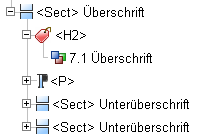
\includegraphics{images/headings}
%		\end{minipage}
%		\hfill
%	\caption{Struktur für Überschriften}
%	\label{fig:headings}
%\end{figure}
%
%
%\subsection{Hilfsmakro}
% %%%%%%%%%%%%%%%%%%%%%
%
%\begin{environment}{PDFSect}
%Beginnt ein neues Strukturelement, aber nur in dem Fall, dass die Option \optname{highstructure} gesetzt ist. Anschließend wird ein spezielles Textobjekt (H) begonnen, und die Absatzmarkierung konfiguriert.
%    \begin{macrocode}
\newenvironment{PDFSect}[2]{%
  \ifPDFDetailedStructure%
      \closeUntilPDFStruct{#1}%
      \PDFStructObj{#1}{#2}%
  \fi%
  \PDFSpezialTextObj{H}%
  \EveryparConfig{H}{false}%
}%
%    \end{macrocode}
%Am Ende der überschrift wird nur die Markierung der Textpassage und das Textobjekt beendet. Die Struktur beginnt ja mit der erst. Sie wird bei Beginn einer höherliegenden Gliederungsebene geschlossen.
%    \begin{macrocode}
{%
  \endPDFMarkContent%
  \endPDFSpezialTextObj%
}
%    \end{macrocode}

%\end{environment}
%
%
%Nachdem nun die abstrakten Hilfsmakros angelegt sind, können die betroffenen Gliederungsbefehle umdefiniert werden.
%
%\subsection{Kapitel}
% %%%%%%%%%%%%%%%%%%%%%
%
%Da der Gliederungsbefehl für Kapitel nur in einigen Dokumentenklassen angeboten wird, ist hierzu eine Sonderbehandlung nötig. Für die verschiedenen Aufrufe ist zudem ist eine Fallunterscheidung nötig.
%
%\subsubsection{Umdefinieren des chapter-Befehls}
% %%%%%%%%%%%%%%%%%%%%%%%%
%
%\begin{macro}{chapter}
%Das Umdefinieren des \comname{chapter}-Befehls.
%    \begin{macrocode}
\ifthenelse{\boolean{@Access@pdf}}{%
  \@ifundefined{chapter}{% es gibt keine Chapter z.B. in Article-Klassen
    }{%
    \let\originalchapter\chapter%
    \renewcommand{\chapter}{%Sortiert die verschiedenen Aufrufe
      \@ifstar{\originalchapterWithStar}%\chapter*{Beispielkapitel}
      {\@ifnextchar[%]
          {\originalchapterWithTwoOption}%\chapter[BspKap]{Beispielkapitel}
          {\originalchapterWithOption}%\chapter{Beispielkapitel}
      }%
    }%
  }%
}{}
%    \end{macrocode}

%Zuordnung der verschiedenen Aufrufvarianten.
%    \begin{macrocode}
\newcommand{\originalchapterWithStar}[1]{%
  \PDFSect{Chapter}{#1}\originalchapter*{#1}\endPDFSect}%
\newcommand{\originalchapterWithTwoOption}[2]{%
  \PDFSect{Chapter}{#1}\originalchapter[#1]{#2}\endPDFSect}%
\newcommand{\originalchapterWithOption}[1]{%
  \PDFSect{Chapter}{#1}\originalchapter{#1}\endPDFSect}%
%    \end{macrocode}

%\end{macro}
%
%\begin{macro}{addchap}
%Das Umdefinieren des \comname{addchap}-Befehls.
%    \begin{macrocode}
\ifthenelse{\boolean{@Access@pdf}}{%
  \@ifundefined{addchap}{% es gibt keine Chapter z.B. in Article-Klassen
  }{%
    \let\originaladdchap\addchap%
    \renewcommand{\addchap}{%
      \@ifstar{\originaladdchapWithStar}%
      {\@ifnextchar[%]
          {\originaladdchapWithTwoOption}%
          {\originaladdchapWithOption}%
      }%
    }%
  }%
}{}
%    \end{macrocode}

%Zuordnung der verschiedenen Aufrufvarianten.
%    \begin{macrocode}
\newcommand{\originaladdchapWithStar}[1]{%
  \PDFSect{Chapter}{#1} \originaladdchap*{#1} \endPDFSect}%
\newcommand{\originaladdchapWithTwoOption}[2]{%
  \PDFSect{Chapter}{#1} \originaladdchap[#1]{#2} \endPDFSect}%
\newcommand{\originaladdchapWithOption}[1]{%
  \PDFSect{Chapter}{#1} \originaladdchap{#1} \endPDFSect}%
%    \end{macrocode}
%\end{macro}

%Im KOMA-Script gibt es die Möglichkeit eine Präamble für Kapeitel und Parts zu setzten. Diese wird durch die nächsten Zeilen als \pdfname{P} ausgezeichnet.
%
%    \begin{macrocode}
\ifthenelse{\boolean{@Access@pdf}}{%
  \@ifundefined{set@preamble}{% es gibt kein set@preamble%
    }{%  %außerhalb des KOMA-Scripts
    \let\originaluse@preamble\use@preamble%
    \renewcommand{\use@preamble}[1]{%
        \EveryparConfig{P}{true}%
        \originaluse@preamble{#1}%
        \EveryparConfig{H}{false}%
    }%
  }%
}{}
%    \end{macrocode}

%\subsection{Überschriften mit Afterskip}
% %%%%%%%%%%%%%%%%%%%%%%%%
%
%Diese Gliederungsebenen gibt es in allen Dokumentenklassen.
%
%\begin{macro}{section}
%Umdefinieren des \comname{section}-Befehls
%    \begin{macrocode}
\ifthenelse{\boolean{@Access@pdf}}{%
  \let\originalsection\section%
  \renewcommand{\section}{%
    \@ifstar{\originalsectionWithStar}%
    {\@ifnextchar[%]
        {\originalsectionWithTwoOption}%
        {\originalsectionWithOption}%
    }%
  }%
}{}
%    \end{macrocode}

%Zuordnung der verschiedenen Aufrufvarianten.
%    \begin{macrocode}
\newcommand{\originalsectionWithStar}[1]%
  {\PDFSect{Section}{#1} \originalsection*{#1} \endPDFSect}%
\newcommand{\originalsectionWithTwoOption}[2]%
  {\PDFSect{Section}{#1} \originalsection[#1]{#2} \endPDFSect}%
\newcommand{\originalsectionWithOption}[1]%
  {\PDFSect{Section}{#1} \originalsection{#1} \endPDFSect}%
%    \end{macrocode}

%\end{macro}
%
%\begin{macro}{subsection}
%Umdefinieren des \comname{subsection}-Befehls
%    \begin{macrocode}
\ifthenelse{\boolean{@Access@pdf}}{%
  \let\originalsubsection\subsection%
  \renewcommand{\subsection}{%
    \@ifstar{\originalsubsectionWithStar}%
    {\@ifnextchar[%]
        {\originalsubsectionWithTwoOption}%
        {\originalsubsectionWithOption}%
    }%
  }%
}{}
%    \end{macrocode}

%Zuordnung der verschiedenen Aufrufvarianten.
%    \begin{macrocode}
\newcommand{\originalsubsectionWithStar}[1]%
  {\PDFSect{Subsection}{#1} \originalsubsection*{#1} \endPDFSect}%
\newcommand{\originalsubsectionWithTwoOption}[2]%
  {\PDFSect{Subsection}{#1} \originalsubsection[#1]{#2} \endPDFSect}%
\newcommand{\originalsubsectionWithOption}[1]%
  {\PDFSect{Subsection}{#1} \originalsubsection{#1} \endPDFSect}%
%    \end{macrocode}

%\end{macro}
%\begin{macro}{subsection}
%Umdefinieren des \comname{subsubsection}-Befehls
%    \begin{macrocode}
\ifthenelse{\boolean{@Access@pdf}}{%
  \let\originalsubsubsection\subsubsection%
  \renewcommand{\subsubsection}{%
    \@ifstar{\originalsubsubsectionWithStar}%
      {\@ifnextchar[%]
        {\originalsubsubsectionWithTwoOption}%
        {\originalsubsubsectionWithOption}%
    }%
  }%
}{}
%    \end{macrocode}

%Zuordnung der verschiedenen Aufrufvarianten.
%    \begin{macrocode}
\newcommand{\originalsubsubsectionWithStar}[1]%
  {\PDFSect{Subsubsection}{#1} \originalsubsubsection*{#1} \endPDFSect}%
\newcommand{\originalsubsubsectionWithTwoOption}[2]%
  {\PDFSect{Subsubsection}{#1} \originalsubsubsection[#1]{#2} \endPDFSect}%
\newcommand{\originalsubsubsectionWithOption}[1]%
  {\PDFSect{Subsubsection}{#1} \originalsubsubsection{#1} \endPDFSect}%
%    \end{macrocode}

%\end{macro}
%
%
%\subsection{Überschriften ohne Afterskip}
% %%%%%%%%%%%%%%%%%%%%%%%%
%In der im scrrept-Definierten Überschriftsvariante werden \comname{paragraph} und \comname{subparagraph} ohne nachfolgenden Zeilenumbruch gesetzt. Solche Überschriften werden als Textabschnitt gekennzeichnet.
%
%\begin{environment}{PDFParagraphSect}
%
%Nachdem wieder ein Strukturobjekt erzeugt wurde. Beginnt \comname{PDFTextObj} ein normales TextObjekt. Die Markierung des ContentStreams muss in diesem Fall explizit geöffnet werden, da die Überschrift durch \comname{everypar} vor den Absatz gesetzt wird und somit nicht richtig erkannt wird. %    \begin{macrocode}
\newenvironment{PDFParSect}[2]{%
  %\ifPDFDetailedStructure%
  %    \closeUntilPDFStruct{#1}%
  %    \PDFStructObj{#1}{#2}%
  %\fi%
  \PDFTextObj%
  \EveryparConfig{P}{false}%
  \PDFMarkContent%
}%
%    \end{macrocode}
%Die Erkennung des Endes kann \comname{everypar} aber durchaus überlassen werden. An dieser Stelle wäre die Beendigung zu früh und würde zu einer leeren Markierung führen.
%    \begin{macrocode}
{%
  %\endPDFMarkContent% erst durch everypar
  %\endPDFTextObj%
}
%    \end{macrocode}

%\end{environment}
%
%\begin{macro}{paragraph}
%Umdefinieren des \comname{paragraph}-Befehls
%    \begin{macrocode}
\ifthenelse{\boolean{@Access@pdf}}{%
  \let\originalparagraph\paragraph%
  \renewcommand{\paragraph}{%
    \@ifstar{\originalparagraphWithStar}%
    {\@ifnextchar[%]
        {\originalparagraphWithTwoOption}%
        {\originalparagraphWithOption}%
    }%
  }%
}{}
%    \end{macrocode}

%Zuordnung der verschiedenen Aufrufvarianten.
%    \begin{macrocode}
\newcommand{\originalparagraphWithStar}[1]%
  {\PDFParSect{Paragraph}{#1} \originalparagraph*{#1}	\endPDFParSect}%
\newcommand{\originalparagraphWithTwoOption}[2]%
  {\PDFParSect{Paragraph}{#1} \originalparagraph[#1]{#2}	\endPDFParSect}%
\newcommand{\originalparagraphWithOption}[1]%
  {\PDFParSect{Paragraph}{#1} \originalparagraph{#1}	\endPDFParSect}%
%    \end{macrocode}

%\end{macro}
%\begin{macro}{subparagraph}
%Umdefinieren des \comname{subparagraph}-Befehls
%    \begin{macrocode}
\ifthenelse{\boolean{@Access@pdf}}{%
  \let\originalsubparagraph\subparagraph%
  \renewcommand{\subparagraph}{%
    \@ifstar{\originalsubparagraphWithStar}%
    {\@ifnextchar[%]
        {\originalsubparagraphWithTwoOption}%
        {\originalsubparagraphWithOption}%
    }%
  }%
}{}
%    \end{macrocode}

%Zuordnung der verschiedenen Aufrufvarianten.
%    \begin{macrocode}
\newcommand{\originalsubparagraphWithStar}[1]%
  {\PDFParSect{Subparagraph}{#1} \originalsubparagraph*{#1}	\endPDFParSect}%
\newcommand{\originalsubparagraphWithTwoOption}[2]%
  {\PDFParSect{Subparagraph}{#1} \originalsubparagraph[#1]{#2}	\endPDFParSect}%
\newcommand{\originalsubparagraphWithOption}[1]%
  {\PDFParSect{Subparagraph}{#1} \originalsubparagraph{#1}	\endPDFParSect}%
%    \end{macrocode}

%\end{macro}
%\subsection{Minisec}
% %%%%%%%%%%%%%%%%%%%%%%%%
%Ein wenig getrennt von den anderen Überschriften ist die im Koma-Script-Paket eingeführt \comname{minisec}. Sie generiert eine kleine Zwischenüberschrift und wird nicht ins Inhaltsverzeichnis aufgenommen. Sie soll (mittels H) als solche gekennzeichnet werden. Die eigentliche Markierung übernimmt \comname{everypar}.
%
%\begin{macro}{minisec}
%Umdefinieren des \comname{mnisec}-Befehls
%    \begin{macrocode}
\ifthenelse{\boolean{@Access@pdf}}{%
  \@ifundefined{minisec}{}{%
   \let\originalminisec\minisec%
   \renewcommand{\minisec}{%
     \@ifstar{\originalminisecWithStar}%
     {\@ifnextchar[%]
         {\originalminisecWithTwoOption}%
         {\originalminisecWithOption}%
     }%
   }%
  }%
}{}
%    \end{macrocode}

%Zuordnung der verschiedenen Aufrufvarianten.
%    \begin{macrocode}
\newcommand{\originalminisecWithStar}[1]%
  {\PDFSpezialTextObj{H}\EveryparConfig{H}{false}%
        \originalminisec*{#1} \endPDFSpezialTextObj}%
\newcommand{\originalminisecWithTwoOption}[2]%
  {\PDFSpezialTextObj{H}\EveryparConfig{H}{false}%
        \originalminisec[#1]{#2} \endPDFSpezialTextObj}%
\newcommand{\originalminisecWithOption}[1]%
  {\PDFSpezialTextObj{H}\EveryparConfig{H}{false}%
        \originalminisec{#1} \endPDFSpezialTextObj}%
%    \end{macrocode}

%\end{macro}
%
%
% %%%%%%%%%%%%%%%%%%%%%%%%%%%%%%%%%%%%%%%%%%%%%%%%%%%%%%%%%%%%%%%%%%%
%\section{Blockelemente}
% %%%%%%%%%%%%%%%%%%%%%%%%
%
%Blockelemente sind Strukturen wie Zitatumgebungen. Sie bestehen aus einer besonderen Textumgebung, die spezielle Abschnitte logisch hervorhebt.
%
%\subsection{Zitatumgebungen}
% %%%%%%%%%%%%%%%%%%%%%%%%
%
%Für Zitatumgebungen steht, in den Standardelementen von PDF, nur das \pdfname{Quote}-Objekt zur Verfügung. Es ist ein spezielles Textobjekt wodurch auch eine Schachtelung von Elementen auf Zeilenebene möglich ist. Den Standardfall ohne weitere Schachtelungen zeigt  Abbildung \ref{fig:quote}.

%\begin{figure}[htbp]
%		\hfill
%		\begin{minipage}[t]{0.40\columnwidth}%
%		\minisec{Die Latex-Struktur}\vspace{\lineheight}
%		\begin{verbatim}
%		\begin{quote}
%		 "Ich bin ein
%		  kurzes Zitat."
%		\end{quote}
%		\end{verbatim}
%		\end{minipage}
%		\hfill
%		\begin{minipage}[t]{0.40\columnwidth}%
%		\minisec{Die PDF-Struktur}\vspace{\lineheight}
%		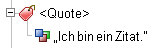
\includegraphics{images/quote}
%		\end{minipage}
%		\hfill
%	\caption{Struktur einer Zitatumgebung}
%	\label{fig:quote}
%\end{figure}
%
%
%\subsubsection{Das eigentliche Umdefinieren}
% %%%%%%%%%%%%%%%%%%%%%%%%
%    \begin{macrocode}
\ifthenelse{\boolean{@Access@pdf}}{%
%    \end{macrocode}
%\begin{environment}{quote}
%Umdefinieren der \comname{quote}-Umgebung
%    \begin{macrocode}
  \let\originalquote\quote%
  \let\originalendquote\endquote%
  \renewenvironment*{quote}%
    {\PDFSpezialTextObj{Quote}\EveryparConfig{Quote}{false}\originalquote}%
    {\endPDFMarkContent\originalendquote\endPDFSpezialTextObj}%
%    \end{macrocode}
%\end{environment}
%\begin{environment}{quotation}
%Umdefinieren der \comname{quotation}-Umgebung
%    \begin{macrocode}
  %
  \let\originalquotation\quotation%
  \let\originalendquotation\endquotation%
  \renewenvironment*{quotation}%
    {\PDFSpezialTextObj{Quote}\EveryparConfig{Quote}{false}\originalquotation}%
    {\endPDFMarkContent\originalendquotation\endPDFSpezialTextObj}%
%    \end{macrocode}
%\end{environment}
%\begin{environment}{verse}
%Umdefinieren der \comname{verse}-Umgebung
%    \begin{macrocode}
  %
  \let\originalverse\verse%
  \let\originalendverse\endverse%
  \renewenvironment*{verse}%
    {\PDFSpezialTextObj{Quote}\EveryparConfig{Quote}{false}\originalverse}%
    {\endPDFMarkContent\originalendverse\endPDFSpezialTextObj}%
}{}
%    \end{macrocode}

%\end{environment}
%
%\subsection{Verbatim, Listings und andere}
% %%%%%%%%%%%%%%%%%%%%%%%%
%In PDF steht eine \pdfname{Code}-Objekt für Computerprogramme und ähnliche Strukturen zur Verfügung. Es soll im folgenden zur Umsetzung der Verbatim-Umgebung herangezogen werden. Bei zukünftigen Umsetzungen von \packname{listings} oder \packname{algorithm} sollte ein ähnliches VorgehLen gewählt werden.
%
%\begin{figure}[htbp]
%		\hfill
%		\begin{minipage}[t]{0.40\columnwidth}%
%		\minisec{Die Latex-Struktur}\vspace{\lineheight}%
%		\begin{verbatim}
%		%begin{verbatim}
%		  Quelltext%
%		%end{verbatim}
%		\end{verbatim}
%		\end{minipage}
%		\hfill
%		\begin{minipage}[t]{0.40\columnwidth}%
%		\minisec{Die PDF-Struktur}\vspace{\lineheight}%
%		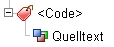
\includegraphics{images/code}%
%		\end{minipage}
%		\hfill
%	\caption{Struktur von Code}
%	\label{fig:code}
%\end{figure}
%
%
%\begin{environment}{verbatim}
%Die folgende Umsetzung funktioniert ohne extra Paket sowie mit den Paketen \packname{verbatim} und \packname{fancyvrb}. Es kommt je verwendeter Verbatim-Umgebung zu einem Fehler ("`Something's wrong--perhaps a missing \string\item."'), allerdings hat dieser keine festgestellten Auswirkungen auf das erzeugte Dokument.
%    \begin{macrocode}
\ifthenelse{\boolean{@Access@pdf}}{%
  \let\originalverbatim\@verbatim%
  \renewcommand{\@verbatim}{%
  %\PDFStructObj{Div}{\empty}%
  \PDFSpezialTextObj{Code}
    \originalverbatim%
  }%
  \let\originalendverbatim\endverbatim%
  \renewcommand{\endverbatim}{%
    \endPDFMarkContent%
    \originalendverbatim%
    \endPDFSpezialTextObj%
    %\endPDFStructObj%
  }%
  \expandafter\let\csname endverbatim*\endcsname =\endverbatim%
}{}
%    \end{macrocode}

%\end{environment}
%
%
%\subsection{Theorem}
% %%%%%%%%%%%%%%%%%%%%%%%%
%
%Theoreme dienen der Verwaltung von Definitionen, Merksätzen, Beispielen, Aufgaben... und transportieren damit wichtige logische Informationen die sich in der Struktur widerspiegeln sollten. Da diese Strukturen aber recht flexibel sind, ist kein rechtes Pendant in der PDF-Spezifikation auszumachen. Anbieten tut sich jedoch das abstrakte \pdfname{Div}-Element von dem eigene Strukturen abgeleitet werden könnten. Eine Wiederverwendung des definierten Stukturnames führt jedoch zu Problemen. Zum Einen ist die Sprache der PDF-Objekte bisher Englisch, während der Theoremname praktisch in allen Sprachen definiert sein kann, was zum Anderen auch zu Problemen mit Sonderzeichen(z.~B. Umlaute, Akzente...) führt. Daher werden Theoreme vorerst als \pdfname{Div} umgesetzt.
%
%\begin{figure}[htbp]
%		\hfill
%		\begin{minipage}[t]{0.40\columnwidth}%
%		\minisec{Die Latex-Struktur}\vspace{\lineheight}
%		\begin{verbatim}
%		\begin{definition}
%		  Ein Theorem ...
%		\end{definition}
%		\end{verbatim}
%		\end{minipage}
%		\hfill
%		\begin{minipage}[t]{0.40\columnwidth}%
%		\minisec{Die PDF-Struktur}\vspace{\lineheight}
%		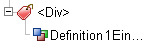
\includegraphics{images/theorem}
%		\end{minipage}
%		\hfill
%	\caption{Struktur eines Theorems}
%	\label{fig:theorem}
%\end{figure}
%
%Poteniell schachtelbar mit z.~B. Itemize oder mehrere Absätze.
%\begin{TODO} vielleicht Argumente auswerten, zur extra Kennzeichnung als heading\end{TODO}
%\begin{TODO} vielleicht Name in Title übernehmen mit pdfstring\end{TODO}
%
%\begin{environment}{theorem}
%Umdefinieren der \comname{theorem}-Umgebung.
%    \begin{macrocode}
\ifthenelse{\boolean{@Access@pdf}}{%
%    \end{macrocode}
%überprüfung ob das Paket thmbox geladen ist.
%    \begin{macrocode}
  \@ifpackageloaded{thmbox}{%
    \PackageWarning{accessibility}%
        {The thmbox-package isn't yet supported.}%
  }{}%
%    \end{macrocode}
%Umdefinieren von theroem, wenn das theorem-Paket geladen ist.
%    \begin{macrocode}
  \@ifpackageloaded{theorem}{%
    \newcommand{\@myendtheorem}{%
      \@endtheorem%
      \endPDFSpezialTextObj%
    }%TODO ungetestet
    \let\original@thm\@thm%
    \gdef\@thm#1#2{%
      \PDFSpezialTextObj{Div}%
      \EveryparConfig{H}{true}%
      \PDFMarkContent%
      \global \expandafter \let \csname end#1\endcsname \@myendtheorem%
      \original@thm{#1}{#2}%
    }%
%    \end{macrocode}
%Umdefinieren von theroem ohne das theorem-Paket
%    \begin{macrocode}
  }{%without theorem-package
    \let\original@begintheorem\@begintheorem%
    \renewcommand{\@begintheorem}{%
      \PDFSpezialTextObj{Div}%
      \EveryparConfig{H}{true}%
      \PDFMarkContent%
      \EveryparConfig{P}{true}%
      \original@begintheorem%
    }%
    \let\original@opargbegintheorem\@opargbegintheorem%
    \renewcommand{\@opargbegintheorem}{%
      \PDFSpezialTextObj{Div}%
      \EveryparConfig{H}{true}%
      \PDFMarkContent%
      \EveryparConfig{P}{true}%
      \original@opargbegintheorem%
    }%
    \let\original@endtheorem\@endtheorem%
    \renewcommand{\@endtheorem}{%
      \original@endtheorem%
      \endPDFSpezialTextObj%
%
    }%
  }%
}{}
%    \end{macrocode}

%\end{environment}
%
%\subsection{Aufzählumgebungen}
% %%%%%%%%%%%%%%%%%%%%%%%%
%Bei Aufzählungen sieht es im Vergleichzu den Zitatumgebungen schon etwas komplizierter aus. Da in \LaTeX\ standardmäßig bis zu vier Schachtelungen erlaubt sind.
%
%Wie bei den Zitatumgebungen existiert in PDF laut Spezifikation nur eine Listenstruktur \pdfname{L}. Sie unterliegt einer festen Gliederung (vgl. Abbildung \ref{fig:list}). Wobei jeder Listeneintrag \pdfname{LI} aus einem optionalen Label \pdfname{Lbl} und einem obligatorischen Listenkörper \pdfname{LBody} besteht.
%
%\begin{figure}[htbp]
%		\hfill
%		\begin{minipage}[t]{0.40\columnwidth}%
%		\minisec{Die Latex-Struktur}\vspace{\lineheight}
%		\begin{verbatim}
%		\begin{description}
%		  \item[Begriff 1] erster Punkt
%		  \item[Begriff 2] zweiter Punkt
%		\end{description}
%		\end{verbatim}
%		\end{minipage}
%		\hfill
%		\begin{minipage}[t]{0.40\columnwidth}%
%		\minisec{Die PDF-Struktur}\vspace{\lineheight}
%		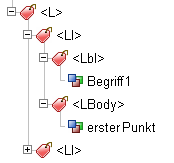
\includegraphics{images/liste}
%		\end{minipage}
%		\hfill
%	\caption{Struktur einer Liste}
%	\label{fig:list}
%\end{figure}
%
%Geschachtelte Unterlisten sind auf der Ebene des /LI der übergeordneten einzugliedern.
%
%\subsubsection{Variablendeklaration}
% %%%%%%%%%%%%%%%%%%%%%%%%
%Im folgenden werden einige Variablen benötigt, um die Elemente zusammenzusetzen sowie die Ebenen zu Unterscheiden.
%    \begin{macrocode}
\newif\ifItemActive \ItemActivefalse%
\newcounter{ListDepth}%
%    \end{macrocode}

%
%\subsubsection{Hilfsmakros}
% %%%%%%%%%%%%%%%%%%%%%%%%
%
%\begin{environment}{PDFList}
%Dieses Makro initialisiert im einfachsten Fall nach der Beendigung des noch aktiven Textes nur die Liste. D.~h. die Variablen werden initialisiert bzw. zurückgesetzt, sollte zuvor schon eine Liste abgearbeitet worden sein. Für den Fall, dass schon einer Liste offen ist, soll in dieser noch das letzte Item abgeschlossen werden. Ausserdem muss der Befehl |\item| für eine Erkennung umdefiniert werden.
%    \begin{macrocode}
\newenvironment{PDFList}{%
  \ifItemActive \closeItem\fi%
  %Liste beginnen
  \addtocounter{ListDepth}{1}%
  %\PDFStructObj{L}{\empty}% Sonst Fehler bei Zugriffsprüfung AA
  \PDFStructObj{L\arabic{ListDepth}}{\empty}%
  %\PDFStructObj{L\romannumeral\theListDepth}{\empty}%
}{%
  \ifItemActive \closeItem\fi%
  %Liste beenden
  \endPDFStructObj%
  \addtocounter{ListDepth}{-1}%
}
%    \end{macrocode}

%\end{environment}
%
%\begin{environment}{PDFListLabel}
%Diese Umgebung klammert den \comname{item} Befehl und kennzeichnet somit das Label. Da der \pdfname{LBody} in \LaTeX\ nicht explizit ausgezeichnet ist, wird nach Abschluss des Labels gleich mit dem \pdfname{LBody} fortgesetzt.
%    \begin{macrocode}
\newenvironment{PDFListLabel}{%
  \ifItemActive \closeItem\fi%
  \PDFStructObj{LI}{\empty}%
  \global\ItemActivetrue%
  \PDFSpezialTextObj{Lbl}%
  \EveryparConfig{Lbl}{false}%
  \PDFMarkContent%
}{%
  \endPDFMarkContent%
  \endPDFSpezialTextObj%
  \PDFSpezialTextObj{LBody}%
  \EveryparConfig{LBody}{false}%
  %\PDFMarkContent{LBody}% wird über everypar erledigt
}%
%    \end{macrocode}

%\end{environment}
%
%\begin{macro}{\closeItem}
%Ein zugehöriges Gegenstück, wie bei anderen Befehlen gibt es aufgrund der \LaTeX-Struktur nicht. Somit sollte zu Beginn eines neuen Items oder am Ende der Liste das letzte Item geschlossen werden. Diese Funktionalität kapselt dieses Makro.
%    \begin{macrocode}
\newcommand{\closeItem}{%		Altes Item abschließen
  \endPDFMarkContent%
  \endPDFSpezialTextObj%{LBody}
  \endPDFStructObj%
  \global\ItemActivefalse%
}
%    \end{macrocode}

%\end{macro}
%
%\subsubsection{Das eigentliche Umdefinieren}
% %%%%%%%%%%%%%%%%%%%%%%%%
%    \begin{macrocode}
\ifthenelse{\boolean{@Access@pdf}}{%
%    \end{macrocode}
%\begin{environment}{itemize}
%Umdefinieren der itemize-Umgebung
%    \begin{macrocode}
  \let\originalitemize\itemize%
  \let\originalenditemize\enditemize%
  \renewenvironment{itemize}%
    {\begin{PDFList}\originalitemize}%
    {%\ifItemActive \closeItem\fi%
     \originalenditemize\end{PDFList}}%
  %
%    \end{macrocode}
%Kennzeichnung der Label für Itemize.
%    \begin{macrocode}
  \let\originallabelitemi\labelitemi%
  \renewcommand{\labelitemi}{%
     \begin{PDFListLabel} \originallabelitemi	\end{PDFListLabel}}%
  \let\originallabelitemii\labelitemii%
  \renewcommand{\labelitemii}{%
     \begin{PDFListLabel} \originallabelitemii	\end{PDFListLabel}}%
  \let\originallabelitemiii\labelitemiii%
  \renewcommand{\labelitemiii}{%
     \begin{PDFListLabel} \originallabelitemiii	\end{PDFListLabel}}%
  \let\originallabelitemiv\labelitemiv%
  \renewcommand{\labelitemiv}{%
     \begin{PDFListLabel} \originallabelitemiv	\end{PDFListLabel}}%
  %
%    \end{macrocode}
%\end{environment}
%\begin{environment}{enumerate}
%Umdefinieren der enumerate-Umgebung
%    \begin{macrocode}
  \let\originalenumerate\enumerate%
  \let\originalendenumerate\endenumerate%
  \renewenvironment{enumerate}%
    {\begin{PDFList}\originalenumerate}%
    {%\ifItemActive \closeItem\fi%
     \originalendenumerate\end{PDFList}}%
  %
%    \end{macrocode}
%Kennzeichnung der Label für Enumerate.
%    \begin{macrocode}
  \let\originallabelenumi\labelenumi%
  \renewcommand{\labelenumi}{%
    \begin{PDFListLabel} \originallabelenumi	\end{PDFListLabel}}%
  \let\originallabelenumii\labelenumii%
  \renewcommand{\labelenumii}{%
    \begin{PDFListLabel} \originallabelenumii	\end{PDFListLabel}}%
  \let\originallabelenumiii\labelenumiii%
  \renewcommand{\labelenumiii}{%
    \begin{PDFListLabel} \originallabelenumiii	\end{PDFListLabel}}%
  \let\originallabelenumiv\labelenumiv%
  \renewcommand{\labelenumiv}{%
    \begin{PDFListLabel} \originallabelenumiv	\end{PDFListLabel}}%
  %
%    \end{macrocode}
%\end{environment}
%\begin{environment}{description}
%Umdefinieren der description-Umgebung
%    \begin{macrocode}
  \let\originaldescription\description%
  \let\originalenddescription\enddescription%
  \renewenvironment{description}%
    {\begin{PDFList}\originaldescription}%
    {%\ifItemActive \closeItem\fi%
     \originalenddescription\end{PDFList}}%
  %
%    \end{macrocode}
%Kennzeichnung der Label für Description.
%    \begin{macrocode}
  \let\originaldescriptionlabel\descriptionlabel% aus scrrept
  \renewcommand{\descriptionlabel}[1]{%
     \begin{PDFListLabel} \originaldescriptionlabel{#1} \end{PDFListLabel}}%
}{}
%    \end{macrocode}

%\end{environment}
%
%
%\subsection{Formeln}
% %%%%%%%%%%%%%%%%%%%%%%%%
% Das PDF-Element \pdfname{Formula} ist für die Auszeichnung von Formeln gedacht (vgl. Abbildung \ref{fig:formula}). Eine logische Differenzierung in eingebettet und freistehende Formeln wird nicht vorgenommen. Dieses Unterscheidungsmerkmal kann durch die unterschiedliche Einbettung in die Struktur wiedergegeben werden. Zum einen kann das Formelobjekt in den Textabsatz eingegliedert werden, zum anderen unter das aktive Section-Objekt. Wie die Struktur für die Formel selbst auszusehen hat zeigt \autoref{fig:formula}.
%
%\begin{figure}[htbp]
%		\hfill
%		\begin{minipage}[t]{0.40\columnwidth}%
%		\minisec{Die Latex-Struktur}\vspace{\lineheight}
%		\begin{verbatim}
%		\(
%		  \alt{c^2=a^2+b^2}
%		  c^{2}=a^{2}+b^{2}
%		\)
%		\end{verbatim}
%		\end{minipage}
%		\hfill
%		\begin{minipage}[t]{0.40\columnwidth}%
%		\minisec{Die PDF-Struktur}\vspace{\lineheight}
%		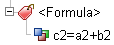
\includegraphics{images/formula}
%		\end{minipage}
%		\hfill
%	\caption{Struktur einer Formel}
%	\label{fig:formula}
%\end{figure}
%
%
%\subsubsection{Das eigentliche Umdefinieren}
% %%%%%%%%%%%%%%%%%%%%%%%%
%\begin{TODO} alle Formeltypen und Alt-Tag\end{TODO}
%    \begin{macrocode}
\ifthenelse{\boolean{@Access@pdf}}{%
%    \end{macrocode}
%\begin{environment}{\[\]}
%Hier wird die Formelumgebungen, die durch eckige Klammern gekennzeichnet wird ausgezeichnet.
%    \begin{macrocode}
  \let\originalFormulaBegin\[%
  \renewcommand*{\[}{%
      \PDFSpezialTextObj{Formula}
      \EveryparConfig{Formula}{false}%%
      \originalFormulaBegin%
  }%
  \let\originalFormulaEnd\]%
  \renewcommand*{\]}{%
      \endPDFMarkContent
      \originalFormulaEnd%
      \endPDFSpezialTextObj%
  }%
%    \end{macrocode}
%\end{environment}
% Die Formelumgebung \comname{math} greift intern auf |\(\)| zu, ebenso wie \comname{displaymath} auf |\[\]|, dadurch brauchen diese Umgebungstypen nicht extra behandelt werden.
%
%Um den komplexeren Formelumgebungen wirklich gerecht zu werden, sollten sie eventuell in mehrere Formeln zerlegt und dann in die Struktur eingebunden werden.
%
%\begin{environment}{equation}
%Im Folgenden wird die equation-Umgebung gekapselt.
%    \begin{macrocode}
  \let\originalequation\equation%
  \let\originalendequation\endequation%
  \renewenvironment{equation}%
    {\PDFSpezialTextObj{Formula}\EveryparConfig{Formula}{false}\originalequation}%
    {\endPDFMarkContent\originalendequation\endPDFSpezialTextObj}%
    %
%    \end{macrocode}
%\end{environment}
%
%\begin{environment}{eqnarray}
%Auszeichnung des eqnarray, dabei wurde auf eine Umsetzung der Tabelle absichtlich verzichtet, diese dient eher der Darstellung, als der logischen Gliederung.
%    \begin{macrocode}
  \let\originaleqnarray\eqnarray%
  \let\originalendeqnarray\endeqnarray%
  \renewenvironment{eqnarray}%
   {%\def&{\originalamp}%  --> das bringt den Fehler inaccessibile
    \PackageWarning{accessibilty}{The `eqnarray` environment should not be used anymore. It is deprecated.}%
     \PDFSpezialTextObj{Formula}%
     \EveryparConfig{Formula}{false}\originaleqnarray}%
   {\endPDFMarkContent\originalendeqnarray\endPDFSpezialTextObj}%
}{}%
%    \end{macrocode}

%\end{environment}
%
%
%
% %%%%%%%%%%%%%%%%%%%%%%%%%%%%%%%%%%%%%%%%%%%%%%%%%%%%%%%%%%%%%%%%%%%
%\subsection{Gleitumgebungen}
% %%%%%%%%%%%%%%%%%%%%%%%%
%
%Da Gleitumgebungen (Figure, Float) werden von \LaTeX\ positioniert werden und können möglicherweise auf einer anderen Seite landen. Die zugehörigen Seitenobjekte, die in /Pg angegeben werde, sollten bei der Definition dynamisch berechnet werden.
%
%Eine Gleiumgebung (z.B. eine Abbildung, Tabelle oder ein Listing) sollte entsprechend der Abbildung \ref{fig:figure} umgesetzt werden. Es ist allerdings darauf zu achten, dass \comname{includegraphics} und ähnliche Befehle auch ohne Gleitumgebung auftauchen können und z.~B. in einer \comname{figure}-Gleitumgebung keinesfalls nur eindeutige Grafikbefehle verwandt werden können. Hier könnten auch einfacher Text oder eine Minipage enthalten sein. Deshalb wird zur Umsetzung eine eigens definiertes \pdfname{Float}-Tag verwendet, dass von \pdfname{Div} abgeleitet ist. Die geschachtelten Grafiken, Tabellen, Captions werden dieser \pdfname{Float}-Struktur untergeordnet. Dies ist die stabilere Lösung, da \comname{includegraphics} oder \comname{tabular} auch ohne zugehöriges Gleitobjekt auftreten kann.
%
%\begin{figure}[htbp]
%		\hfill
%		\begin{minipage}[t]{0.40\columnwidth}%
%		\minisec{Die Latex-Struktur}\vspace{\lineheight}
%		\begin{verbatim}
%		\begin{figure}[htbp]
%		  \alt{Ich bin das Logo der
%		      Technischen Universität}
%		  
\includegraphics{/tu_logo}
%		  \caption{TU-Logo}
%		\end{figure}
%		\end{verbatim}
%		\end{minipage}
%		\hfill
%		\begin{minipage}[t]{0.40\columnwidth}%
%		\minisec{Die PDF-Struktur}\vspace{\lineheight}
%		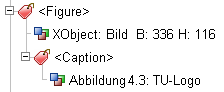
\includegraphics{images/figure}
%		\end{minipage}
%		\hfill
%	\caption{Struktur einer Grafik}
%	\label{fig:figure}
%\end{figure}
%
%
%\begin{environment}{float}
% Umdefinieren der float-Umgebung, diese wird sowohl füür die Definition von \comname{figure}und \comname{table} als auch für selbstdefinierte Floatumgebungen verwendet.
%    \begin{macrocode}
\ifthenelse{\boolean{@Access@pdf}}{%
  \let\original@float\@float%
  \let\originalend@float\end@float%
  \renewenvironment*{@float}[1]{%
    \PDFStructObj{Float}{\csname #1name\endcsname}%
    %\global\numberingparsfalse%
    \original@float{#1}%
  }{%
    \originalend@float%
    \endPDFMarkContent%
    %\global\numberingparstrue%
    \endPDFStructObj%
  }%
}{}
%    \end{macrocode}

%\end{environment}
%
%\subsection{Caption}
% %%%%%%%%%%%%%%%%%%%%%%%%
%
% Eine Bildunterschrift (CM)tritt normalerweise in einer Gleitumgebung auf. Der Befehl kann allerdings auch in einer minipage oder irgendwo anders verwendet werden.
%\begin{macro}{caption}
%Durch das umdefinieren von \comname{@makecaption} funktioniert diese Umsetzung mit den Standardklassen, den Klassen des KOMA-Scriptes sowie mit dem \packname{caption}-Paket.
%    \begin{macrocode}
\ifthenelse{\boolean{@Access@pdf}}{%
  \let\original@@makecaption\@makecaption%
 %  \renewcommand{\@makecaption}[3]{%
  \renewcommand{\@makecaption}[2]{%
    \global\numberingparsfalse%
    \PDFSpezialTextObj{Caption}%
    \EveryparConfig{Caption}{false}%
    \PDFMarkContent%
      \PackageWarning{accessibility}{begin makecaption}%
%        \original@@makecaption{#1}{#2}{#3}%
      \original@@makecaption{#1}{#2}%{#3}%
      \PackageWarning{accessibility}{end makecaption}%
    \endPDFMarkContent%
    \endPDFSpezialTextObj%{Caption}%
    \global\numberingparstrue%
  }%
}{}
%    \end{macrocode}

%\end{macro}
%
%|\captionbelow|
%|\captionbeside|
%|\captionabove|
%
%
%\subsection{Tabellen}
% %%%%%%%%%%%%%%%%%%%%%%%%
%
%Eine Tabelle besteht in PDF aus drei großen Teilen, dem Tabellenkopf, dem -körper und dem -fuß. Diese bestehen jeweils aus Tabellenreihe, die wiederum Tabellendatenzellen bzw. Tabellenüberschriftszellen enthalten.
%
%Eine Unterscheidung in Kopf, Körper und Fuß ist in \LaTeX-Tabellen nicht zu finden. Lediglich die Erweiterung \packname{longtable} bringt ein ähnliches Konzept mit.
%
%\begin{figure}[htbp]
%		\hfill
%		\begin{minipage}[t]{0.40\columnwidth}%
%		\minisec{Die Latex-Struktur}\vspace{\lineheight}
%		\begin{verbatim}
%		\begin{table}[htbp]
%		  \begin{tabular}{l|l l}
%		    \thead{11} & \thead{12} &
%		    \thead{13} \\ \hline
%		    21 & 22 & 23 \\
%		    31 & 32 & 33 \\
%		  \end{tabular}
%		  \caption{meine Tabelle}
%		\end{table}
%		\end{verbatim}
%		\end{minipage}
%		\hfill
%		\begin{minipage}[t]{0.40\columnwidth}%
%		\minisec{Die PDF-Struktur}\vspace{\lineheight}
%		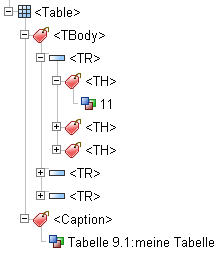
\includegraphics{images/table}
%		\end{minipage}
%		\hfill
%	\caption{Struktur einer Tabelle}
%	\label{fig:table}
%\end{figure}
%
% %\subsubsection{Variablendeklaration}
% %%%%%%%%%%%%%%%%%%%%%%%%
%
%    \begin{macrocode}
\newif\ifTableHeadCell \global\TableHeadCellfalse%
\newif\ifTableLineActive \global\TableLineActivefalse%
\newif\ifTableCellActive \global\TableCellActivefalse%
\newif\ifAfterKill \global\AfterKillfalse%
%    \end{macrocode}

%
% %\subsubsection{Hilfsmakro}
% %%%%%%%%%%%%%%%%%%%%%%%%
%
%\begin{environment}{PDFTable} Umschließt die gesamte Tabelle.
%    \begin{macrocode}
\newenvironment{PDFTable}{%
  \global\numberingparsfalse%
  \PDFStructObj{Table}{\empty}%
  \PDFStructObj{TBody}{\empty}%
  \global\TableLineActivefalse%
  \global\TableCellActivefalse%
}{%
  \ifTableLineActive\endPDFTableLine\fi%
  \endPDFStructObj%{TBody}{\empty}%
  \endPDFStructObj%{Table}{\empty}%
  \global\numberingparstrue%
}%
%    \end{macrocode}

%\end{environment}
%
%\begin{environment}{PDFTableLine} Eine Tabellenzeile
%    \begin{macrocode}
\newenvironment{PDFTableLine}{%
  \ifTableCellActive\endPDFTableCell\fi%
  \ifTableLineActive\endPDFTableLine\fi%
  \global\TableLineActivetrue%
  \PDFStructObj{TR}{\empty}%
}{%
  \ifTableLineActive%
    \endPDFStructObj%
    \global\TableLineActivefalse%
  \fi%
}%
%    \end{macrocode}

%\end{environment}
%
%\begin{environment}{PDFTableCell} Eine Tabellenzelle, die Unterscheidung in Überschrifts- und Datenzelle wird vom Autor getroffen. Der zugrunde liegende Wahrheitswert wird in \varname{TableHeadCell} gespeichert.
%
%    \begin{macrocode}
\newenvironment{PDFTableCell}{%
  \ifTableCellActive\endPDFTableCell\fi%
  \global\TableCellActivetrue%
  \PDFSpezialTextObj{TD}%
  \EveryparConfig{TD}{false}%
  \PDFMarkContent%
}{%
  \ifTableCellActive%
    \endPDFMarkContent%
    \ifTableHeadCell%
       \xdef\TextType{TH}%
       \global\TableHeadCellfalse%
    \fi%
    \endPDFSpezialTextObj%{TD}%
    \global\TableCellActivefalse%
  \fi%
}%
%    \end{macrocode}

%\end{environment}
%
%\subsubsection{Das eigentliche Umdefinieren}
% %%%%%%%%%%%%%%%%%%%%%%%%
%\begin{environment}{tabular}
%Umdefinieren der \comname{tabular}-Umgebung.
%    \begin{macrocode}
\def\originalamp{&}%
\catcode`\&=\active%
\def&{\originalamp}%

\ifthenelse{\boolean{@Access@pdf}}{%
  \let\originaltabular\tabular%
  \let\originalendtabular\endtabular%
  \renewenvironment*{tabular}{%
    \def&{\endPDFTableCell\originalamp\PDFTableCell}%
    \PDFTable%
    \PDFTableLine%
    \PDFTableCell%
    %%%%%%%%%%%%%%%%%%%%%%%%%%%%%%%%%%%%%%%%%%%%%%%%%
    \originaltabular%
  }{%
    %\pdfliteral{EMC}%
    \def&{\originalamp}%
    \originalendtabular%
    %%%%%%%%%%%%%%%%%%%%%%%%%%%%%%%%%%%%%%%%%%%%%%%%%
    \ifTableCellActive\endPDFTableCell\fi%
    \ifTableLineActive\endPDFTableLine\fi%
    \endPDFTable%
  }%
%    \end{macrocode}
%\end{environment}
%Zur Markierung des Tabellenzeilenendes, es ist eine Unterscheidung nötig, je nachdem, ob das Paket \packname{tabularx} geladen ist oder nicht.
%    \begin{macrocode}
  \@ifpackageloaded{array}{%
    \let\originalaryend\@arraycr%
    \renewcommand*{\@arraycr}{\endPDFTableCell%
       \endPDFTableLine\PDFTableLine\PDFTableCell\originalaryend}%
  }{% wenn kein anderes Tabellen-Package
    \let\originaltabend\@tabularcr%
    \renewcommand*{\@tabularcr}{\endPDFTableCell%
       \endPDFTableLine\PDFTableLine\PDFTableCell\originaltabend}%
  }%
%    \end{macrocode}
%Die Pakete \packname{tabularx} und {longtable} sowie weitere werden bisher nicht behandelt.
%    \begin{macrocode}
 % \@ifpackageloaded{tabularx}{%
 %   \PackageWarning{accessibity}%
 %       {The tabularx-package isn't yet fully supported.%
 %        You can use the tabular-environemt but not the tabularx.}
 % }{}%
 % \@ifpackageloaded{longtable}{%
 %   \PackageWarning{accessibity}%
 %        {The longtable-package isn't yet supported.}
 %   %\tabularnewline  \endhead\endfirsthead\endfoot\endlastfoor
 % }{}%
}{}%
%    \end{macrocode}

%\begin{environment}{tabbing}
%Umdefinieren der \comname{tabbing}-Umgebung.
%    \begin{macrocode}
\ifthenelse{\boolean{@Access@pdf}}{%
  \let\originaltabbing\tabbing%
  \let\originalendtabbing\endtabbing%
  \renewenvironment*{tabbing}{%
    \PDFTable%
    \let\originalkill\kill%
    \renewcommand{\kill}{\global\AfterKilltrue%
      \originalkill%%
    }%
    %%%%%%%%%%%%%%%%%%%%%%%%%%%%%%%%%%%%%%%%%%%%%%%%%
    \originaltabbing%
  }{%
    \originalendtabbing%
    %%%%%%%%%%%%%%%%%%%%%%%%%%%%%%%%%%%%%%%%%%%%%%%%%
    \endPDFTable%
  }%
  \let\original@startfield\@startfield%
  \renewcommand{\@startfield}{%
    \original@startfield \ifAfterKill\PDFTableCell\fi%
  }%
  \let\original@stopfield\@stopfield%
  \renewcommand{\@stopfield}{%
    \ifAfterKill\endPDFTableCell\fi \original@stopfield%
  }%
  \let\original@startline\@startline%
  \renewcommand{\@startline}{%
    \ifAfterKill\PDFTableLine\fi \original@startline%
  }%
  \let\original@stopline\@stopline%
  \renewcommand{\@stopline}{%
    \original@stopline \ifAfterKill\endPDFTableLine\fi%
  }%
}{}
%    \end{macrocode}

%\end{environment}
%
% %%%%%%%%%%%%%%%%%%%%%%%%%%%%%%%%%%%%%%%%%%%%%%%%%%%%%%%%%%%%%%%%%%%
%\section{Elemente auf Zeilenebene}
% %%%%%%%%%%%%%%%%%%%%%%%%
%
%
%\subsection{Texthervorhebungen}
% %%%%%%%%%%%%%%%%%%%%%%%%
% Zeichnet Formatierungen im Fließtext als /Span aus, um sie gesondert hervorzuheben. Eine Auszeichnung von reinen Textdekorationen (z.B. |\textbf{}|, |\textit{}| ...) ist hierbei jedoch fraglich, da sie auch in Makros verwendet werden und somit möglicherweise mehrfach ausgezeichnet werden, was zum einen zu Problemen in der Struktur führt und zum anderen schnell unübersichtlich wird. Vergleichbare Elemente sind in PDF nicht vorgesehen und auch in XHTML 2.0 soll die Trennung vonn Inhalt und Layout durch den Wegfall der Elemente (|<b>|,|<it>| ...) vollendet werden.
%
%Hingegen transportiert die Struktur |\emph{}| durchaus semantische Informationen. Nämlich das der Text hervorgehoben ist.
%
%\subsubsection{Das eigentliche Umdefinieren}
% %%%%%%%%%%%%%%%%%%%%%%%%

%\begin{macro}{emph}
%Die Auszeichnung des \comname{emph}-Befehls.
%    \begin{macrocode}
\ifthenelse{\boolean{@Access@pdf}}{%
  \let\originalemph\emph%
  \renewcommand{\emph}[1]{%
    \begin{PDFInlineObjInText}{Span}%
    \originalemph{#1}%
    \end{PDFInlineObjInText}%
  }%
}{}
%    \end{macrocode}

%\end{macro}
%
% %%%%%%%%%%%%%%%%%%%%%%%%%%%%%%%%%%%%%%%%%%%%%%%%%%%%%%%%%%%%%%%%%%%
%\subsection{Verweise auf andere Textstellen}
% %%%%%%%%%%%%%%%%%%%%%%%%
%Für Verweise auf anderen Textstellen bietet PDF die Struktur \pdfname{Reference}.
%
%\begin{figure}[htbp]
%		\hfill
%		\begin{minipage}[t]{0.40\columnwidth}%
%		\minisec{Die Latex-Struktur}\vspace{\lineheight}
%		\begin{verbatim}
%		...S.
%		\pageref
%		...
%		\end{verbatim}
%		\end{minipage}
%		\hfill
%		\begin{minipage}[t]{0.40\columnwidth}%
%		\minisec{Die PDF-Struktur}\vspace{\lineheight}
%		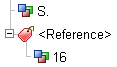
\includegraphics{images/reference}
%		\end{minipage}
%		\hfill
%	\caption{Die Struktur einer Referenz}
%	\label{fig:reference}
%\end{figure}
%
%    \begin{macrocode}
\ifthenelse{\boolean{@Access@pdf}}{%
%    \end{macrocode}
%Wenn das hyperref-Paket geladen ist.
%    \begin{macrocode}
  \@ifpackageloaded{hyperref}{%
    \let\original@setref\@setref%
    \renewcommand{\@setref}[3]{%
        \begin{PDFInlineObjInText}{Reference}%
        \original@setref{#1}{#2}{#3}%
        \end{PDFInlineObjInText}}%
    %Linkziele%
    %\let\originalhyper@anchorstart\hyper@anchorstart%
    %\renewcommand{\hyper@anchorstart}%
    %{\pdfliteral{/Span <</E (anchorstart)>> BDC EMC}%
    %\originalhyper@anchorstart}%
    %\let\originalhyper@anchorend\hyper@anchorend%
    %\renewcommand{\hyper@anchorend}{\originalhyper@anchorend
    %\pdfliteral{/Span <</E (anchorend)>> BDC EMC}}%
    % Einträge im TOC, LOF, LOT
    %\let\originalhyper@linkstart\hyper@linkstart%
    %\renewcommand{\hyper@linkstart}{%
    %    \begin{PDFInlineObjInText}{Reference}%
    %     \originalhyper@linkstart}%
    %\let\originalhyper@linkend\hyper@linkend%
    %\renewcommand{\hyper@linkend}{%
    %     \originalhyper@linkend%
    %    \end{PDFInlineObjInText}}%
    %\useacronym --> Kurzform, Glossarseitezahlen,
    %Indexseitenzahlen, Glossareinträge, Hyperlink
    \let\originalhyperlink\hyperlink%
    \renewcommand*{\hyperlink}[2]{%
        \ifIndexItemActive\else\begin{PDFInlineObjInText}{Reference}\fi%
        %Wenn Index -- folgender Aufruf
        % hyperlink{page.\the\toks@}{\the\toks@}%
        %Bringt Fehler
        \originalhyperlink{#1}{#2}%\relax%
        \ifIndexItemActive\else\end{PDFInlineObjInText}\fi%
    }%
    %href  pdfobleme mit pdf 1.3 \@urlbordercolor nicht definiert
    \let\originalhyper@linkurl\hyper@linkurl%
    \renewcommand{\hyper@linkurl}[2]{%
        \begin{PDFInlineObjInText}{Link}%
        \originalhyper@linkurl{#1}{#2}%
        \end{PDFInlineObjInText}}%
    %
    \let\originalhyper@linkfile\hyper@linkfile%
    \renewcommand{\hyper@linkfile}[3]{%
        \begin{PDFInlineObjInText}{Link}%
        \originalhyper@linkfile{#1}{#2}{#3}%
        \end{PDFInlineObjInText}}%
    %Seitenzahlen in Index, anders da anschließend
    %keine Texterkennung nötig.
    %eigentlich über hyperlink möglich
    \let\originalhyperpage\hyperpage%
    \renewcommand{\hyperpage}[1]{%
        \EveryparConfig{Reference}{true}%
        \PDFMarkContent% kein everypar
        \originalhyperpage{#1}%
        \endPDFMarkContent}%
    % URL
    \let\originalnolinkurl\nolinkurl%
    \renewcommand{\nolinkurl}[1]{%
        \begin{PDFInlineObjInText}{Link}%
        \originalnolinkurl{#1}%
        \end{PDFInlineObjInText}}%
%    \end{macrocode}
%Wenn das hyperref-Paket nicht geladen ist.
%    \begin{macrocode}
  }{%	ohne hyperref
%    \end{macrocode}
% Umdefinieren des \comname{ref}-Befehls
%    \begin{macrocode}
      \let\originalref\ref%
      \renewcommand{\ref}[1]{%
        \begin{PDFInlineObjInText}{Reference}%
        \originalref{#1}%
        \end{PDFInlineObjInText}}%
      %
%    \end{macrocode}
% Umdefinieren des \comname{pageref}-Befehls
%    \begin{macrocode}
      \let\originalpageref\pageref%
      \renewcommand{\pageref}[1]{%
        \begin{PDFInlineObjInText}{Reference}%
        \originalpageref{#1}%
        \end{PDFInlineObjInText}}%
  }%
}{}
%    \end{macrocode}
%
%Diese Umsetzung funktioniert auch mit dem \packname{varioref}-Paket, da dieses intern auf die Definitionen von \comname{ref} bzw. \comname{pageref}. Die korrekte Auszeichnung sowie die Einbindung der Referenzen funktioniert auch wenn das \packname{hyperref}-Paket geladen ist.
%
%
%\begin{macro}{cite}
%Umdefinieren des \comname{cite}-Befehls, der auf das Literaturverzeichnis verweist.
%    \begin{macrocode}
\ifthenelse{\boolean{@Access@pdf}}{%
  \let\originalcite\cite%
  \renewcommand{\cite}[2][__empty__]{% #1 Name des Eintages
    \begin{PDFInlineObjInText}{Reference}%
    \ifthenelse{\equal{#1}{__empty__}}%
        {\originalcite{#2}}%
        {\originalcite[#1]{#2}}%
    \end{PDFInlineObjInText}%
  }%
}{}
%    \end{macrocode}

%Eine getrennte Auszeichnung der Glossareninträge ist nicht mehr nötig. Das \packname{glossary} greift auf \comname{hyperlink} zurück. Auch möglich Seitenbezüge im Glossar werden über \comname{hyperlink} aktivert.
%\end{macro}
%
% %%%%%%%%%%%%%%%%%%%%%%%%%%%%%%%%%%%%%%%%%%%%%%%%%%%%%%%%%%%%%%%%%%%
%\subsection{eingebettete Objekte im Textfluss}
% %%%%%%%%%%%%%%%%%%%%%%%%
%
%\begin{macro}{\verb}
%An dieser Stelle erfolgt das Umdefinieren der eingebetteten Codeumgebung, die durch \comname{verb} gekennzeichnet wird.
%    \begin{macrocode}
\ifthenelse{\boolean{@Access@pdf}}{%
  \let\originalverb\verb%
  \renewcommand{\verb}{%
    \begin{PDFInlineObjInText}{Code}%
    \originalverb%
  }%
  \let\originalverb@egroup\verb@egroup%
  \renewcommand{\verb@egroup}{%
   \originalverb@egroup%
    \end{PDFInlineObjInText}%
  }%
}{}
%    \end{macrocode}

%\end{macro}
%
%\begin{environment}{\(\)}
%An dieser Stelle erfolgt das Umdefinieren der eingebetteten Formelumgebungen, die durch runde Klammern gekennzeichnet wird.
%    \begin{macrocode}
  \let\originalFormulaTextBegin\(%
  \renewcommand*{\(}{%
      \PDFInlineObjInText{Formula}%
      \originalFormulaTextBegin%
  }%
  \let\originalFormulaTextEnd\)%
  \renewcommand*{\)}{%
      \originalFormulaTextEnd%
      \endPDFInlineObjInText%
  }%
%    \end{macrocode}

%\end{environment}

%
%\subsection{Fußnoten}
% %%%%%%%%%%%%%%%%%%%%%%%%
%
%Eine Fußnote besteht generell aus zwei Bestandteilen, der Markierung im Text (footnotemark) und der eigentlichen Fußnote am Seitenende (footnotetext). Beide Teile müssen sinnvoll in die Struktur eingegliedert werden. Hierzu wird die Lesereihenfolge der Elemente im Strukturbaum geändert, sodass der Text an Ort und Stelle verfögbar ist und nicht erst am Seitenende (nach "`zig"' Absätzen) vorgelesen wird (vgl. Abbildung \ref{fig:footnote}).
%
%\begin{figure}[htbp]
%		\hfill
%		\begin{minipage}[t]{0.40\columnwidth}%
%		\minisec{Die Latex-Struktur}\vspace{\lineheight}
%		\begin{verbatim}
%		...Fußnote
%		\footnote{Fußnotentext}
%		...
%		\end{verbatim}
%		\end{minipage}
%		\hfill
%		\begin{minipage}[t]{0.40\columnwidth}%
%		\minisec{Die PDF-Struktur}\vspace{\lineheight}
%		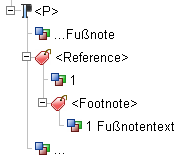
\includegraphics{images/footnote}
%		\end{minipage}
%		\hfill
%	\caption{Fußnotenstruktur im Absatz}
%	\label{fig:footnote}
%\end{figure}
%
%\begin{TODO} Fußnoten außerhalb von Text sind im Moment nicht vorgesehen. $\rightarrow$ Flexibilisierung der Schachtelung. Also z.B. in Tabelle, überschrift ... \end{TODO}
%
%\subsubsection{Variablendeklaration}
% %%%%%%%%%%%%%%%%%%%%%%%%
%    \begin{macrocode}
\newcounter{PDFFootnotemark}%
\newcounter{PDFFootnotetext}%
\newcounter{ObjNum}
%    \end{macrocode}

%
%\subsubsection{Hilfsmakros}
% %%%%%%%%%%%%%%%%%%%%%%%%
%\begin{environment}{PDFFootnote} umschließt die gesamte Fußnotenstruktur.
%    \begin{macrocode}
\newenvironment{PDFFootnote}{%
  \global\numberingparsfalse%
  \pdfobj reserveobjnum%
  \setcounter{PDFFootnotemark}{\pdflastobj}%
  \pdfobj reserveobjnum%
  \setcounter{PDFFootnotetext}{\pdflastobj}%
}{%
  %\EveryparConfig{\lastEveryparType}{\HelpBool}%
  \global\numberingparstrue%
  \EveryparConfig{\lastEveryparType}{false}%
  \PDFMarkContent%
}
%    \end{macrocode}

%\end{environment}
%
%\begin{environment}{PDFFootnoteReference} Die eigentliche Referenz auf die Fußnote im Text. Sie setzt sich aus dem markierten Inhalt (MCID) und der Fußnote am Seitenende zusammen.
%    \begin{macrocode}
\newenvironment{PDFFootnoteReference}{%
    \xdef\HelpBool{\InlineObj}%
    \EveryparConfig{Reference}{obj}%
    \setcounter{ObjNum}{\theTaggedObj}%
    \PDFMarkContent%
}{%
    \endPDFMarkContent%
    \writeComplexTextObj{\thePDFFootnotemark}%
        {\theObjNum \space \thePDFFootnotetext \space 0 R}%
        {/Reference}{\theTextObjNum}{Page}%
    \xdef\TextArray{\TextArray \theObjHelp\space 0 R \space}%
}
%    \end{macrocode}

%\end{environment}
%
%\begin{environment}{PDFFootnoteText}Die eigentliche Fußnote am Seitenende. Sie wird als Kind der Fußnotenreferenz in den Strukturbaum eingefügt.
%    \begin{macrocode}
\newenvironment{PDFFootnoteText}{%
   \EveryparConfig{Note}{obj}%
   \setcounter{ObjNum}{\theTaggedObj}%
   \PDFMarkContent%
}{%
   \endPDFMarkContent%
   \writeComplexTextObj%
          {\thePDFFootnotetext}{\theObjNum}%
          {/Footnote}{\thePDFFootnotemark}{Page}%
}
%    \end{macrocode}

%\end{environment}
%
%\subsubsection{Das eigentliche Umdefinieren}
% %%%%%%%%%%%%%%%%%%%%%%%%
% Die Befehle stammen aus der soure2e-Dokumentation.
%    \begin{macrocode}
\ifthenelse{\boolean{@Access@pdf}}{%
%    \end{macrocode}
%Umdefinieren der \comname{footnotemark}
%    \begin{macrocode}
  \let\original@footnotemark\@footnotemark%
  %Fußnotenreferenz im Text
  \renewcommand{\@footnotemark}{%
    \begin{PDFFootnoteReference}%
    \original@footnotemark%
    \end{PDFFootnoteReference}%
  }%
%    \end{macrocode}
%Umdefinieren der \comname{footnotetext}
%    \begin{macrocode}
  \let\original@makefntext\@makefntext%
  %Fußnotentext am Seitenende
  \renewcommand{\@makefntext}[1]{%
    \begin{PDFFootnoteText}%
    \original@makefntext{#1}%
    \end{PDFFootnoteText}%
  }%
%    \end{macrocode}
%Umdefinieren der gesamten Fußnote \comname{footnote}
%    \begin{macrocode}
  \let\originalfootnote\footnote%
  \def\footnote{\@ifnextchar[{\@@xxfootnote}{\@@xfootnote}}%
  \def\@@xxfootnote[#1]#2{%
    \begin{PDFFootnote}%
    \originalfootnote[#1]{#2}%
    \end{PDFFootnote}%
  }%
  \def\@@xfootnote#1{%
    \begin{PDFFootnote}%
    \originalfootnote{#1}%
    \end{PDFFootnote}%
  }%
}{}
%    \end{macrocode}

%
%
%
% %%%%%%%%%%%%%%%%%%%%%%%%%%%%%%%%%%%%%%%%%%%%%%%%%%%%%%%%%%%%%%%%%%%
%\section{Verzeichnisse}
% %%%%%%%%%%%%%%%%%%%%%%%%
% Zahlreiche Verzeichnisse stehen in \LaTeX\ zur Verfügung. Ihre logische Auszeichnung kann Nutzern assistiver Technologien den Zugang zum Dokument erleichtern.
%\subsection{Inhaltsverzeichnis und die Listen der Float-Objekte}
% %%%%%%%%%%%%%%%%%%%%%%%%
%
%\begin{figure}[htbp]
%		\hfill
%		\begin{minipage}[t]{0.40\columnwidth}%
%		\minisec{Die Latex-Struktur}\vspace{\lineheight}
%		\begin{verbatim}
%		...
%		\tableofcontents
%		    \contentsline {chapter}%
%		    {Abbildungsverzeichnis}%
%		    {3}{chapter*.2}
%		...
%		\end{verbatim}
%		\end{minipage}
%		\hfill
%		\begin{minipage}[t]{0.40\columnwidth}%
%		\minisec{Die PDF-Struktur}\vspace{\lineheight}
%		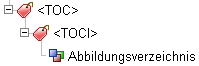
\includegraphics{images/Tocontent}
%		\end{minipage}
%		\hfill
%	\caption{Struktur eines Inhaltsverzeichnisses}
%	\label{fig:Tocontent}
%\end{figure}
%
%
%\subsubsection{Das eigentliche Umdefinieren}
% %%%%%%%%%%%%%%%%%%%%%%%%
%    \begin{macrocode}
\ifthenelse{\boolean{@Access@pdf}}{%
  \let\original@starttoc\@starttoc%
  \renewcommand{\@starttoc}[1]{%
    \ifthenelse{\equal{#1}{toc}}{% Table of content
        \PDFSpezialTextObj{TOC}\EveryparConfig{TOCI}{true}%
    }{}%
    \ifthenelse{\equal{#1}{lot}}{% List of Tables
        \PDFSpezialTextObj{TOT}\EveryparConfig{TOTI}{true}%
    }{}%
    \ifthenelse{\equal{#1}{lof}}{% List of figures
        \PDFSpezialTextObj{TOF}\EveryparConfig{TOFI}{true}%
    }{}%
    %\ifthenelse{\equal{#1}{brf}}{}}{}% Bibliography
    \original@starttoc{#1}%
    \ifthenelse{\equal{#1}{toc} \or \equal{#1}{lot} \or \equal{#1}{lof}}{%
      \endPDFMarkContent%
      \endPDFSpezialTextObj%
    }{}%
  }%
}{}
%    \end{macrocode}

%Verschieben des \comname{endPDFMarkContent}, damit wird es am Ende der letzten Seite und nicht erst oben auf der neuen ausgeführt.
%    \begin{macrocode}
\ifthenelse{\boolean{@Access@pdf}}{%
  \let\originalcontentsline\contentsline
  \@ifpackageloaded{hyperref}{%then: Mit hyperref
    \renewcommand{\contentsline}[4]{%
        \originalcontentsline{#1}{#2}{#3\protect\endPDFMarkContent}{#4}%
    }%
  }{%else: ohne Hyperref
    \renewcommand{\contentsline}[3]{%
        \originalcontentsline{#1}{#2}{#3\protect\endPDFMarkContent}%
   }%
  }%
}{}
%    \end{macrocode}

%
%
%\subsection{Literaturverzeichnis}
% %%%%%%%%%%%%%%%%%%%%%%%%
%
%Das Literaturverzeichnis (Bibliography) besteht aus einzelnen Literaturverzeichniseinträgen (BibEntry), die im Fließtext mit Literaturverweisen referenziert werden können.
%
%\begin{figure}[htbp]
%		\hfill
%		\begin{minipage}[t]{0.40\columnwidth}%
%		\minisec{Die Latex-Struktur}\vspace{\lineheight}
%		\begin{verbatim}
%		\begin{thebibliography}{AFF99}
%		  \bibitem[AFF99]{ansorge:1999}...
%		\end{thebibliography}
%		\end{verbatim}
%		\end{minipage}
%		\hfill
%		\begin{minipage}[t]{0.40\columnwidth}%
%		\minisec{Die PDF-Struktur}\vspace{\lineheight}
%		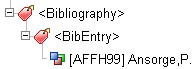
\includegraphics{images/bibliography}
%		\end{minipage}
%		\hfill
%	\caption{Struktur des Literaturverzeichnisses}
%	\label{fig:bibliography}
%\end{figure}
%
%
%\subsubsection{Variablendeklaration}
% %%%%%%%%%%%%%%%%%%%%%%%%
%    \begin{macrocode}
\newif\ifBibItemActive \BibItemActivefalse%
%    \end{macrocode}
%
%\subsubsection{Das eigentliche Umdefinieren}
% %%%%%%%%%%%%%%%%%%%%%%%%
%Die gewählte Variante funktioniert sowohl mit als auch ohne BibTeX.
%
%Umdefinieren der umschließenden \comname{thebibliography}-Umgebung.
%    \begin{macrocode}
\ifthenelse{\boolean{@Access@pdf}}{%
  \let\originalthebibliography\thebibliography%
  \let\originalendthebibliography\endthebibliography%
  \renewenvironment{thebibliography}{%
      \originalthebibliography%
      %\PDFStructObj{Bibliography}% geht hier nicht in bibitem realisiert
  }{%
      \originalendthebibliography%
      \endPDFMarkContent%
      \endPDFSpezialTextObj%{\LBody}
      \endPDFStructObj%{\BibItem}
      \global\BibItemActivefalse%
      \endPDFStructObj%{Bibliography}
  }%
}{}
%    \end{macrocode}

%Umdefinieren des \comname{bibitem}-Befehls.
%    \begin{macrocode}
\ifthenelse{\boolean{@Access@pdf}}{%
  \let\originalbibitem\bibitem%
  \renewcommand{\bibitem}[2][__empty__]{% #1 [Label] #2 Eintrag
    \ifBibItemActive% schon welche
      \endPDFMarkContent%
      \endPDFSpezialTextObj%{\LBody}
      \endPDFStructObj%{\BibItem}
      \global\BibItemActivefalse%
    \else% erstes Item
      \PDFStructObj{Bibliography}{\empty}%
    \fi%
    \global\BibItemActivetrue%
    \PDFStructObj{BibItem}{\empty}%
    \PDFSpezialTextObj{Lbl}%
    \EveryparConfig{Lbl}{false}%
    \PDFMarkContent%
    \ifthenelse{\equal{#1}{__empty__}}%
        {\originalbibitem{#2}}%
        {\originalbibitem[#1]{#2}}%
    %\endPDFMarkContent% Zu früh, Text wird erst mit everypar gestetzt
    \endPDFSpezialTextObj%
    \PDFSpezialTextObj{LBody}%
    \EveryparConfig{LBody}{false}%
   %\PDFMarkContent{LBody}% wird über everypar erledigt
  }%
}{}
%    \end{macrocode}
%
%
%\subsection{Index}
% %%%%%%%%%%%%%%%%%%%%%%%%
%
%Das Stichwortverzeichnis geht häufig über mehrere Spalten und Seiten.
%\begin{TODO}Dabei ist der Umbruch unbedingt zu beachten. $\rightarrow$ Was passiert derzeit?\end{TODO}
%
%\begin{figure}[htbp]
%		\hfill
%		\begin{minipage}[t]{0.40\columnwidth}%
%		\minisec{Die Latex-Struktur}\vspace{\lineheight}
%		\begin{verbatim}
%		\begin{theindex}
%		  \item B\"achlein, 17
%		\end{theindex}
%		\end{verbatim}
%		\end{minipage}
%		\hfill
%		\begin{minipage}[t]{0.40\columnwidth}%
%		\minisec{Die PDF-Struktur}\vspace{\lineheight}
%		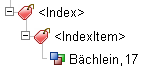
\includegraphics{images/index}
%		\end{minipage}
%		\hfill
%	\caption{Struktur des Index}
%	\label{fig:index}
%\end{figure}
%
%\subsubsection{Variablendeklaration}
% %%%%%%%%%%%%%%%%%%%%%%%%
%    \begin{macrocode}
\newif\ifIndexItemActive \IndexItemActivefalse%
%    \end{macrocode}

%
%\subsubsection{Das eigentliche Umdefinieren}
% %%%%%%%%%%%%%%%%%%%%%%%%
%Umdefinieren der umschließenden \comname{theindex}-Umgebung.
%\begin{TODO}Nur wenn das Paket \packname{index} geladen ist.\end{TODO}
%    \begin{macrocode}
\ifthenelse{\boolean{@Access@pdf}}{%
  \let\originaltheindex\theindex%
  \let\originalendtheindex\endtheindex%
  \renewenvironment{theindex}{%
    \expandafter\originaltheindex\relax%
  }{%
      \endPDFMarkContent%
    \originalendtheindex%
    \ifIndexItemActive%
      \endPDFSpezialTextObj%
      \global\IndexItemActivefalse%
    \fi
    \endPDFStructObj%{Index}%
  }%
}{}
%    \end{macrocode}

%Umdefinieren des \comname{@idxitem}-Befehls.
%    \begin{macrocode}
\ifthenelse{\boolean{@Access@pdf}}{%
  \let\original@idxitem\@idxitem%
  \renewcommand*\@idxitem{%
    \ifIndexItemActive% schon welche
      \endPDFMarkContent%
      \endPDFSpezialTextObj%
      \global\IndexItemActivefalse%
    \else% erstes Item
      \PDFStructObj{Index}%
    \fi%
    \global\IndexItemActivetrue%
    \PDFSpezialTextObj{IndexEntry}%
    \EveryparConfig{IndexEntry}{false}%
    \original@idxitem%
  }%
}{}
%    \end{macrocode}

%\begin{TODO}subitem und subsubitem getrennt behandeln um die Schachtelung zu erhalten.\end{TODO}
%
%
%
% %%%%%%%%%%%%%%%%%%%%%%%%%%%%%%%%%%%%%%%%%%%%%%%%%%%%%%%%%%%%%%%%%%%
%\section{Layoutbefehle}
% %%%%%%%%%%%%%%%%%%%%%%%%
%
%Befehle, die ausschließlich dem Layout dienen, werden nicht in den Strukturbaum übernommen. Hier ist stattdessen eine Auszeichnung als \pdfname{Artefakt} vorgesehen.
%
%
%
%\subsection{Kopf- und Fußzeilen als Artefakte}
% %%%%%%%%%%%%%%%%%%%%%%%%
%
%Kopf- und Fußzeilen zählen zu den Artefakten, die sich aus der Seitenaufteilung ergeben. Sie sind folglich als solche (/Type /Page) zu kennzeichnen.
%
%\subsubsection{Hilfsmakro}
% %%%%%%%%%%%%%%%%%%%%%%%%
%
%\begin{environment}{PDFPageArtefakt} Umschließende Struktur für ein Artefakt der Seitenaufteilung.
%    \begin{macrocode}
\newenvironment*{PDFPageArtefakt}{%
  \pdfliteral{/Artifact <</Type /Pagination>> BDC}%
}{%
  \pdfliteral{EMC}%
}
%    \end{macrocode}

%\end{environment}
%
%
%\subsubsection{Das eigentliche Umdefinieren}
% %%%%%%%%%%%%%%%%%%%%%%%%
% Da Scrpage optimal mit den Klassen des Koma-Scripts zusammenarbeitet, funktioniert es mit \packname{scrpage2}.
%\begin{TODO}Funktionstüchtigkeit mit fancyheader und Standardklassen\end{TODO}
%    \begin{macrocode}
\ifthenelse{\boolean{@Access@pdf}}{%
   \let\original@thehead\@thehead%
   \renewcommand*{\@thehead}{%
      \ifthenelse{\equal{\original@thehead}{\empty}}{}{%
          \begin{PDFPageArtefakt}%
          \original@thehead%
          \end{PDFPageArtefakt}%
      }%
   }%
   \let\original@thefoot\@thefoot%
   \renewcommand*{\@thefoot}{%
      \ifthenelse{\equal{\original@thefoot}{\empty}}{}{%
          \begin{PDFPageArtefakt}%
          \original@thefoot%
          \end{PDFPageArtefakt}%
       }%
   }%
}{}
%    \end{macrocode}
%
%\subsection{Linien als Artefakte}
% %%%%%%%%%%%%%%%%%%%%%%%%
%Linien und andere dekorative Inhalte sind laut PDF-Spezifikation als /Artefakte auszuzeichnen. Normale Linien werden in Screenreadern nicht vorgelesen. Speziell die automatische Füllstruktur (|\dotfill|) wird aber durch ASCII-Zeichen gesetzt, d.h. sie wird im Screenreader als "`Punkt Punkt ..."' vorgelesen. Dies stört den Lesefluss erheblich.
%
%\subsubsection{Hilfsmakros}
% %%%%%%%%%%%%%%%%%%%%%%%%
%
%\begin{environment}{PDFLayoutArtefakt} Umschließende Struktur für ein Layout-Artefakt.
%\begin{TODO} Kennzeichnung als Artefakt vom Typ /Layout, dazu sollten weitere Parameter (wie die BoundingBox) in angegebene werden, damit zukünftig das Reflow adäquat funktionieren kann. \end{TODO}
%    \begin{macrocode}
\newenvironment*{PDFLayoutArtefakt}{%
  \numberingparsfalse%
  \pdfliteral{/Artifact <</Type /Layout>> BDC}%
}{%
  \pdfliteral{EMC}%
  \numberingparstrue%
}
%    \end{macrocode}

%\end{environment}
%
%\subsubsection{Das eigentliche Umdefinieren}
% %%%%%%%%%%%%%%%%%%%%%%%%
%Anpassen des \comname{dotfill}-Befehls.
%    \begin{macrocode}
\ifthenelse{\boolean{@Access@pdf}}{%
  \let\originaldotfill\dotfill%
  \renewcommand*{\dotfill}{%
    \begin{PDFLayoutArtefakt}%
    \originaldotfill%
    \end{PDFLayoutArtefakt}%
  }%
%    \end{macrocode}
%Anpassen des \comname{footnoterule}-Befehls. Dieser greift auf hrule zurück und bereite Probleme beim generellen Umdefinieren.
%    \begin{macrocode}
  \let\originalfootnoterule\footnoterule%
  \renewcommand*\footnoterule{%
    \let\hrule\originalhrule%
    \begin{PDFLayoutArtefakt}%
    \originalfootnoterule%
    \end{PDFLayoutArtefakt}%
    \let\originalhrule\hrule%
  }%
%    \end{macrocode}
%Anpassen des \comname{hrule}-Befehls.
%    \begin{macrocode}
   %\vrule height1ex depth0pt width1ex
   %\hrule height1ex depth0pt width1ex
   %
   %hrulefill, hline cline, toprule, midrule, bottomrule, cmidrule? greifen auf hrule zu
  %Klappt nicht immer mit Argumentübergabe
  \let\originalhrule\hrule%
  \def\hrule#1#2{%
    \ifthenelse{\equal{#2}{\z@}}{}{\begin{PDFLayoutArtefakt}}%
    \originalhrule#1#2%
    \ifthenelse{\equal{#2}{\z@}}{}{\end{PDFLayoutArtefakt}}%
  }%
%    \end{macrocode}

% Ebenso sollten sämtliche Tabellenrahmen, Linien in Kopf- und Fußzeile oder Die Linie vor den Fußnoten markiert werden. Am sinnvollsten erscheint die Umdeklaration der |\hrule| und |\vrule| Anweisung. Auf diese wird in den meisten Fällen zurückgegriffen.


%    \begin{macrocode}
  %vline (2), @arrayrule(2?) greift auf vrule zu
  %Klappt nicht mit Argumentübergabe
  %\let\originalvrule\vrule%
  %\def\vrule#1#2{%
  %  \begin{PDFLayoutArtefakt}%
  %  \originalvrule#1#2%
  %  \end{PDFLayoutArtefakt}%
%  }%
}{}
%    \end{macrocode}
%Gepunktete Linien, wie sie im Inhaltsverzeichnis mittels \comname{dottedtocline} erzeugt werden, werden auch als solches (nämlich "`Punkt Punkt ...) vorgelesen. Hierzu wurde die Originaldefinition aus soure2e \cite{Brams2000} um die pdfliterale ergänzt, wodurch die Linie als Artefakt gekennzeichnet ist und nicht vorgelesen wird.
%    \begin{macrocode}
\ifthenelse{\boolean{@Access@pdf}}{%
  \def\@dottedtocline#1#2#3#4#5{%
    \ifnum #1>\c@tocdepth \else%
      \vskip \z@ \@plus.2\p@%
      {\leftskip #2\relax \rightskip \@tocrmarg %
      \parfillskip -\rightskip%
      \parindent #2\relax\@afterindenttrue%
      \interlinepenalty\@M%
      \leavevmode%
      \@tempdima #3\relax%
      \advance\leftskip \@tempdima \null\nobreak\hskip -\leftskip%
      {#4}\nobreak%
      \begin{PDFLayoutArtefakt}%
      \leaders\hbox{$\m@th \mkern %
        \@dotsep mu\hbox{.}\mkern \@dotsep	mu$}\hfill%
      \end{PDFLayoutArtefakt}%
      \nobreak%
      \hb@xt@\@pnumwidth{\hfil\normalfont \normalcolor #5}%
      \par}%
    \fi%
  }%
}{}
%    \end{macrocode}

%\subsection{Titelseite}
% %%%%%%%%%%%%%%%%%%%%%%%%
%Die Titelseite ist sehr von der Gestaltungsfreiheit der Autoren geprägt. Die Standardelemente |\title{}|, |\author{}| und weitere werden oft zu layouttechnischen Zwecken verwandt, so dass eine inhaltliche Auszeichnung in den Augen der Autorin wenig Sinn macht. Damit die Strukturen, die im Bereich des Titels auftauchen einen sinnvollen Rahmen bekommen, wird der durch |\maketitle| erzeugte Inhalt in die Struktur \pdfname{Sect} geschachtelt.
%    \begin{macrocode}
\ifthenelse{\boolean{@Access@pdf}}{%
  \let\originalmaketitle\maketitle%
  \renewcommand{\maketitle}{%
    \PDFStructObj{Div}{Titlepage}%
    \EveryparConfig{P}{false}%
    %
    \originalmaketitle%
    \endPDFMarkContent%
    \endPDFStructObj%
  }%
}{}%

%    \end{macrocode}
%
% %%%%%%%%%%%%%%%%%%%%%%%%%%%%%%%%%%%%%%%%%%%%%%%%%%%%%%%%%%%%%%%%%%%
%\section{Verträglichkeit mit anderen Dokumentklassen}
% %%%%%%%%%%%%%%%%%%%%%%%%
%
% %%%%%%%%%%%%%%%%%%%%%%%%%%%%%%%%%%%%%%%%%%%%%%%%%%%%%%%%%%%%%%%%%%%
%\section{Verträglichkeit mit anderen Paketen}
% %%%%%%%%%%%%%%%%%%%%%%%%
%
%\subsection{Das \packname{multicolumn}-Paket}
% %%%%%%%%%%%%%%%%%%%%%%%%
%Wird wie alle anderen Umgebungen unterstützt. Solange sich die gesamte Umgebung auf einer Seite befindet funktioniert alles, wie gehabt. Dass Seitenumbrüche noch nicht zuverlässig erkannt werden können, treten auch hier mögliche Probleme auf. Eine Verwendung sollte nur mit anschließender überprüfung des Ergebnisdokumentes erfolgen.
%
%Die Befehle |\twocolumn| und |\onecolumn| aus \PlainTeX funktionieren mit den gleichen Einschränkungen.
%
%\subsection{Das \packname{graphics}-Paket}
%
%\begin{TODO} Die anderen Befehle des \packname{graphicx}-Paketes. (wrapfigure...)\end{TODO}
%    \begin{macrocode}
\ifthenelse{\boolean{@Access@pdf}}{%
  \@ifpackageloaded{graphicx}{%
    \let\originalincludegraphics\includegraphics%
    \renewcommand{\includegraphics}[2][__empty__]{%
    \global\numberingparsfalse%
     % \PDFInlineObjInText{Figure}%
    \PDFSpezialTextObj{Figure}%
    \EveryparConfig{Figure}{false}%
    \PDFMarkContent%
      \ifthenelse{\equal{#1}{__empty__}}%
          {\originalincludegraphics{#2}}%
          {\originalincludegraphics[#1]{#2}}%
    %  \endPDFInlineObjInText%
    \endPDFMarkContent%
    \endPDFSpezialTextObj%{Figure}%
    \global\numberingparstrue%
    }%
  }{}%
}{}
%    \end{macrocode}

%\subsection{Das \packname{picture}-Paket}
% Da das \packname{picture} die Picture-Umgebung transparent umdefiniert, funktioniert die Auszeichnung sowohl  wenn das Paket geladen ist. Auch die Erweiterungen \packname{trees} zum Zeichnen von binären und tertiären Bäumen, \packname{bar} zum Erstellen vom Balkendiagrammen sowie \packname{curves} zum Zeichnen beliebiger Kurven kann verwendet werden .
%    \begin{macrocode}
\ifthenelse{\boolean{@Access@pdf}}{%
    \let\originalpicture\picture%
    \let\originalendpicture\endpicture%
    \renewenvironment{picture}{%
    \global\numberingparsfalse%
    \PDFSpezialTextObj{Figure}%
    \EveryparConfig{Figure}{false}%
    \PDFMarkContent%
    \originalpicture%
 }{%
    \originalendpicture%
    \endPDFMarkContent%
    \endPDFSpezialTextObj%{Figure}%
    \global\numberingparstrue%
    }%
}{}
%    \end{macrocode}

%\subsection{Das \packname{babel}-Paket}

%\begin{macro}{\convertLanguageInCode}
%Dieses Makro konvertiert den übergebenen Sprachstring |{#1}| in den PDF bekannten Zwei-Buchstaben-Kode. Das Ergebnis wir in der Variablen \varname{LanguageCode} gespeichert.
%    \begin{macrocode}
\newcommand{\convertLanguageInCode}[1]{%
  \gdef\LanguageCode{}%
  \ifthenelse{\equal{#1}{\string danish}}{\gdef\LanguageCode{/Lang(DA)}}{}%
  \ifthenelse{\equal{#1}{\string german}}{\gdef\LanguageCode{/Lang(DE)}}{}%
  \ifthenelse{\equal{#1}{\string ngerman}}{\gdef\LanguageCode{/Lang(DE)}}{}%
  \ifthenelse{\equal{#1}{\string germanb}}{\gdef\LanguageCode{/Lang(DE)}}{}%
  \ifthenelse{\equal{#1}{\string austrian}}{\gdef\LanguageCode{/Lang(DE)}}{}%
  \ifthenelse{\equal{#1}{\string naustrian}}{\gdef\LanguageCode{/Lang(DE)}}{}%
  \ifthenelse{\equal{#1}{\string english}}{\gdef\LanguageCode{/Lang(EN)}}{}%
  \ifthenelse{\equal{#1}{\string USenglish}}{\gdef\LanguageCode{/Lang(EN-US)}}{}%
  \ifthenelse{\equal{#1}{\string american}}{\gdef\LanguageCode{/Lang(EN-US)}}{}%
  \ifthenelse{\equal{#1}{\string UKenglish}}{\gdef\LanguageCode{/Lang(EN-GB)}}{}%
  \ifthenelse{\equal{#1}{\string british}}{\gdef\LanguageCode{/Lang(EN-GB)}}{}%
  \ifthenelse{\equal{#1}{\string canadian}}{\gdef\LanguageCode{/Lang(EN)}}{}%
  \ifthenelse{\equal{#1}{\string australian}}{\gdef\LanguageCode{/Lang(EN)}}{}%
  \ifthenelse{\equal{#1}{\string newzealand}}{\gdef\LanguageCode{/Lang(EN)}}{}%
  \ifthenelse{\equal{#1}{\string finnish}}{\gdef\LanguageCode{/Lang(FI)}}{}%
  \ifthenelse{\equal{#1}{\string french}}{\gdef\LanguageCode{/Lang(FR)}}{}%
  \ifthenelse{\equal{#1}{\string francais}}{\gdef\LanguageCode{/Lang(FR)}}{}%
  \ifthenelse{\equal{#1}{\string canadien}}{\gdef\LanguageCode{/Lang(FR)}}{}%
  \ifthenelse{\equal{#1}{\string acadian}}{\gdef\LanguageCode{/Lang(FR)}}{}%
  \ifthenelse{\equal{#1}{\string italian}}{\gdef\LanguageCode{/Lang(IT)}}{}%
  \ifthenelse{\equal{#1}{\string norsk}}{\gdef\LanguageCode{/Lang(NO)}}{}%
  \ifthenelse{\equal{#1}{\string nynorsk}}{\gdef\LanguageCode{/Lang(NO)}}{}%
  \ifthenelse{\equal{#1}{\string portuges}}{\gdef\LanguageCode{/Lang(PT)}}{}%
  \ifthenelse{\equal{#1}{\string portuguese}}{\gdef\LanguageCode{/Lang(PT)}}{}%
  \ifthenelse{\equal{#1}{\string brazilian}}{\gdef\LanguageCode{/Lang(PT-BR)}}{}%
  \ifthenelse{\equal{#1}{\string brazil}}{\gdef\LanguageCode{/Lang(PT-BR)}}{}%
  \ifthenelse{\equal{#1}{\string swedish}}{\gdef\LanguageCode{/Lang(SV)}}{}%
  \ifthenelse{\equal{#1}{\string spanish}}{\gdef\LanguageCode{/Lang(ES)}}{}%
  	% not surreported in babel:
	% Chinese (/Lang{ZH})
	% Korean (/Lang{KO}).
  \ifthenelse{\equal{\LanguageCode}{}}{%
	% comparing \languagename is tricky. See babel package documentation for more information
	\PackageWarning{accessibility}{The chosen language (#1) is not supported %
		by Adobe Reader 6.0.}%
}{}%
}
%    \end{macrocode}

%\end{macro}
%
%
%\subsubsection{Auszeichnung der Dokumentenhauptsprache}
% %%%%%%%%%%%%%%%%%%%%%%%%
%Am Anfang des eigentlichen Dokumentes wird dann die Hauptsprache des PDF-Dokumentes bestimmt und gesetzt. Zusätzlich wird die aktuelle Sprache initialisiert um bei späteren änderungen wirkliche von Dopplungen zu unterscheiden.
%\begin{TODO}Nur wenn babel geladen wurde.\end{TODO}
%    \begin{macrocode}
\ifthenelse{\boolean{@Access@pdf}}{%
  \AtBeginDocument{%
    \gdef\DocumentLanguage{\languagename}%
    \gdef\ActualLanguage{\languagename}%
    \convertLanguageInCode{\languagename}%
    \pdfcatalog{%										Catalog dictionary of PDF output.
      \LanguageCode%								Setzt die Sprache
    }%
  }%
}{}
%    \end{macrocode}

%\subsubsection{Auszeichnung von Sprachwechseln}
% %%%%%%%%%%%%%%%%%%%%%%%%
%
%\subsubsection{Hilfsmakro}
% %%%%%%%%%%%%%%%%%%%%%%%%
%
%    \begin{macrocode}
\newcommand{\recognizeLanguageChange}[1]{%
  \ifthenelse{\equal{#1}{\ActualLanguage}}{%
     %keine änderung zu vorher
  }{%
     \gdef\ActualLanguage{#1}%
     \convertLanguageInCode{\languagename}}%
  \ifthenelse{\equal{#1}{\DocumentLanguage}}{%
     \global\LanguageDifffalse%
  }{%
     \global\LanguageDifftrue%
  }%
}
%    \end{macrocode}
%
%\begin{macro}{\selectlanguage}
%|\selectlanguage{Sprache}| vollständige Ersetzung bis zum Dokumentende oder der nächsten änderung.
% Wenn die neu aktivierte Sprache von der vorherigen abweicht, wird |LanguageDiff| war und alle nun erzeugen Objekte bekommen ein passendes Sprachattribut.
%    \begin{macrocode}
\ifthenelse{\boolean{@Access@pdf}}{%
  \@ifpackageloaded{babel}{%
    \let\originalselectlanguage\selectlanguage%
    \renewcommand{\selectlanguage}[1]{%
      \originalselectlanguage{#1}%
      \recognizeLanguageChange{#1}%
    }%
%    \end{macrocode}
%\end{macro}
%
%\begin{environment}{otherlanguage}
%Da die Umgebung |otherlanguage| beliebige Befehle enthalten kann, scheint der Autorin eine umschließende Umgebung fehleranfällig, es könnte so unsinnigen Verschachtelungen kommen. So dass hier das gleicht Vorgehen wie bei \comname{selectlanguage} gewählt wurde.
%\begin{TODO} |\begin{otherlanguage}{Sprache}| lokale änderung auch in Sternform \end{TODO}
%\begin{TODO} Am Anfang der Umgebung doppelte Abfrage durch die Wiederverwendung von selectlanguage? sollte eventuell beseitigt werden.\end{TODO}
%    \begin{macrocode}
    \let\originalotherlanguage\otherlanguage%
    \let\originalendotherlanguage\otherlanguage%
    \long\def\otherlanguage#1{%
      \csname selectlanguage \endcsname{#1}%
      \ignorespaces%
      \recognizeLanguageChange{#1}%
    }%
%    \end{macrocode}
%
%    \begin{macrocode}
      \long\def\endotherlanguage{%
      \originalTeX%
      \global\@ignoretrue\ignorespaces%
      \recognizeLanguageChange{\languagename}%
    }%
%    \end{macrocode}
%\end{environment}
%
%\begin{macro}{foreignlanguage}
% Der Befehl \comname{foreignlanguage{Sprache}{Inhalte}} ändert die Sprache nur für kleine Textbereiche, bei denen die Sprachänderung mittels \pdfname{Span} in den ContentStream eingefügt wird. Eine Einordnung in den Strukturbaum kann laut \cite{Adobe2004} entfallen.
%    \begin{macrocode}
    \let\originalforeignlanguage\foreignlanguage%
    \renewcommand{\foreignlanguage}[2]{%
      \convertLanguageInCode{\string #1}%
      \pdfliteral{/Span <<\LanguageCode>> BDC}%
      \originalforeignlanguage{#1}{#2}%
      \pdfliteral{EMC}%
      \convertLanguageInCode{\languagename}%
    }%
  }{}%
}{}
%    \end{macrocode}

%\end{macro}
%
%\subsection{Das \packname{makeidx}-Paket}
%\subsection{Das \packname{glossary}-Paket}
%
%\subsubsection{Glossar}
% %%%%%%%%%%%%%%%%%%%%%%%%%%%%%%%%%%%%%%%%%%%%%%%%%%%%%%%%%%%%%%%%%%%
%Die Optionen \optname{altlist} und \optname{list} des \packname{glossary}-Pakets schreiben die Glossareinträge als Definitionsliste, damit sind die Einträge ausreichend gekennzeichnet.
%
%\begin{TODO}: Die Optionen \optname{super} und \optname{long} schreiben je eine Tabelle, entweder als supertabular oder als longtable -->diese werden derzeit nicht korrekt erkannt \end{TODO}
%
%Es muss nichts umdefiniert werden. Ein Umdefinieren des \comname{glositem} muss nicht stattfinden, da intern auf eine Definitionsliste zu gegriffen wird, was der Autorin von der inhaltlichen Aussage her angemessen erscheint
%
%\subsubsection{Glossareinträge und Referenzen}
% %%%%%%%%%%%%%%%%%%%%%%%%%%%%%%%%%%%%%%%%%%%%%%%%%%%%%%%%%%%%%%%%%%%
%Die im Text verwandten Verweise auf ein Glossareintrag werden mit Hilfe der Funktion \comname{hyperlink} des \packname{hyperref}-Paketes gesetzt. So dass sie bereits zuverlässig erkannt werden.
%
%\subsubsection{Abkürzungen und Akronyme}
% %%%%%%%%%%%%%%%%%%%%%%%%%%%%%%%%%%%%%%%%%%%%%%%%%%%%%%%%%%%%%%%%%%%
%Eine mögliche Auszeichnung und Anwendungsmöglichkeiten für Akronyme und Abkürzungen stellt das Paket \packname{glossary} zur Verfügung. Es ermöglicht das Anlegen eines Abkürzungsverzeichnisses und eine Referenzierung der Langform sowie der Kurzform über kurze Befehle.
%
%Dabei sollte für die Kurzform, jeweils die Langform in die PDF-Struktur übernommen werden, so dass assistive Technologien darauf Zugriff haben.
%
%    \begin{macrocode}
\ifthenelse{\boolean{@Access@pdf}}{%
  \@ifpackageloaded{glossary}{%
    \let\originalnewacronym\newacronym%
    \renewcommand{\newacronym}[4][]{%
  %%%%% Originaldefinition
\ifthenelse{\equal{#1}{}}{\renewcommand\@acrnmcmd{#2}}{%
\renewcommand\@acrnmcmd{#1}}%
    \xdef\expansion{#3}%
\@ifundefined{\@acrnmcmd}{%
\expandafter\newcommand\csname\@acrnmcmd short\endcsname{%
\protect\pdfliteral{/Span <</E (\expansion)>> BDC}%
#2%
\protect\pdfliteral{EMC}%
\protect\glsxspace}%
\expandafter\newcommand\csname\@acrnmcmd @nx@short\endcsname{%
\protect\pdfliteral{/Span <</E (\expansion)>> BDC}%
#2%
\protect\pdfliteral{EMC}}%
\expandafter\newcommand\csname\@acrnmcmd long\endcsname{%
#3\protect\glsxspace}
\expandafter\newcommand\csname\@acrnmcmd @nx@long\endcsname{#3}
\def\@acrn@entry{#4}%
{%
\expandafter\@gls@getdescr\expandafter{\@acrn@entry}%
\let\glodesc\@glo@desc%
\def\glolong{#3}%
\@onelevel@sanitize\glolong
\def\gloshort{\noexpand\acronymfont{#2}}%
\@onelevel@sanitize\gloshort
\expandafter\protected@xdef\expandafter\@acrnamefmt{\@acronymnamefmt}
\expandafter\protected@xdef\expandafter\@acrdesc{\@acronymdescfmt}
}%
\@acr@addtolist{\@acrnmcmd}
\@glo@tb=\expandafter{\@acrn@entry}%
\protected@edef\@acr@glsentry{name={\@acrnamefmt},%
format=glsnumformat,sort={\@acrnmcmd},\the\@glo@tb,%
description={\@acrdesc}}%
\@glo@tb=\expandafter{\@acr@glsentry}%
\newboolean{\@acrnmcmd first}\setboolean{\@acrnmcmd first}{true}
\expandafter\protected@edef\csname \@acrnmcmd\endcsname{%
\noexpand\@ifstar{\csname @s@\@acrnmcmd\endcsname}{%
\csname @\@acrnmcmd\endcsname}}
\ifglshyperacronym % hyperlinks
\expandafter\protected@edef\csname @\@acrnmcmd\endcsname{%
\noexpand\ifthenelse{\noexpand\boolean{\@acrnmcmd first}}{%
\csname\@acrnmcmd @nx@long\endcsname\noexpand\@acrnmins\
(\noexpand\xacronym{\the\@glo@tb}{%
\noexpand\acronymfont{\csname\@acrnmcmd @nx@short\endcsname}%
})\noexpand\unsetacronym{\@acrnmcmd}%
}{\noexpand\xacronym{\the\@glo@tb}{%
\noexpand\acronymfont{\csname\@acrnmcmd @nx@short\endcsname}%
\noexpand\@acrnmins}}\noexpand\glsxspace}
\expandafter\protected@edef\csname @s@\@acrnmcmd\endcsname{%
\noexpand\ifthenelse{\noexpand\boolean{\@acrnmcmd first}}{%
\noexpand\expandafter\noexpand\MakeUppercase
\csname\@acrnmcmd @nx@long\endcsname\noexpand\@acrnmins\
(\noexpand\xacronym{\the\@glo@tb}{%
\noexpand\acronymfont{\csname\@acrnmcmd @nx@short\endcsname}%
})%
\noexpand\unsetacronym{\@acrnmcmd}}{%
\noexpand\xacronym{\the\@glo@tb}{%
\noexpand\acronymfont{\noexpand\expandafter\noexpand\MakeUppercase
\csname\@acrnmcmd @nx@short\endcsname}%
\noexpand\@acrnmins}}\noexpand\glsxspace}
\else % no hyperlinks
\expandafter\protected@edef\csname @\@acrnmcmd\endcsname{%
\noexpand\ifthenelse{\noexpand\boolean{\@acrnmcmd first}}{%
\csname\@acrnmcmd @nx@long\endcsname\noexpand\@acrnmins\
(\noexpand\acronym{\the\@glo@tb}{%
\noexpand\acronymfont{\csname\@acrnmcmd @nx@short\endcsname}%
})\noexpand\unsetacronym{\@acrnmcmd}%
}{\noexpand\acronym{\the\@glo@tb}{%
\noexpand\acronymfont{\csname\@acrnmcmd @nx@short\endcsname}%
\noexpand\@acrnmins}}%
\noexpand\glsxspace}
\expandafter\protected@edef\csname @s@\@acrnmcmd\endcsname{%
\noexpand\ifthenelse{\noexpand\boolean{\@acrnmcmd first}}{%
\noexpand\expandafter
\noexpand\MakeUppercase
\csname\@acrnmcmd @nx@long\endcsname\noexpand\@acrnmins\
(\noexpand\acronym{\the\@glo@tb}{%
\noexpand\acronymfont{\csname\@acrnmcmd @nx@short\endcsname}%
})%
\noexpand\unsetacronym{\@acrnmcmd}}{%
\noexpand\acronym{\the\@glo@tb}{%
\noexpand\acronymfont{\noexpand\expandafter\noexpand\MakeUppercase
\csname\@acrnmcmd @nx@short\endcsname}%
\noexpand\@acrnmins}}\noexpand\glsxspace}
\fi
}{%
\PackageError{glossary}{Command '\expandafter\string
\csname\@acrnmcmd\endcsname' already defined}{%
The command name specified by \string\newacronym already exists.}}}
  %%%%% Originaldefinition
  }{}%
}{}
%    \end{macrocode}

%\subsection{Das \packname{booktabs}-Paket}
%Das \packname{booktabs}-Paket stellt vier neue Befehle für Tabellenlinien zur Verfügung. Bei der Definition wird wiederum auf das Makro \comname{hrule} zurück gegriffen, so dass eine Auszeichnung als Artefakt bereits erledigt wird.
%\subsection{Das \packname{hyperref}-Paket}
%Die Nutzung dieses Pakets ist unter Vorsicht zu genießen.  Die Standard-\LaTeX-Befehle funktionieren auch unter Verwendung des Paketes. Paketeigene Erweiterungen sind größtenteils noch nicht implementiert. Sie konnten bisher nicht vollständig getestet werden.
%\subsection{Das \packname{caption}-Paket}
%Das \packname{caption}-Paket kann mit seinen möglichen Konfigurationsparameter ohne Einschränkung verwendet werden. Die alte Version das \packname{caption2}-Paket ist obsolet und sollte nicht mehr verwendet werden.
%\subsection{Das \packname{tabularx}-Paket}
%Die Nutzung dieses Pakets ist unter Vorsicht zu genießen.  Die Standard-\LaTeX-Befehle funktionieren auch unter Verwendung des Paketes. Paketeigene Erweiterungen sind größtenteils noch nicht implementiert. Sie konnten bisher nicht vollständig getestet werden.
%\subsection{Das \packname{longtabular}-Paket}
%Die Nutzung dieses Pakets ist unter Vorsicht zu genießen.  Die Standard-\LaTeX-Befehle funktionieren auch unter Verwendung des Paketes. Paketeigene Erweiterungen sind größtenteils noch nicht implementiert. Sie konnten bisher nicht vollständig getestet werden.
%\subsection{Das \packname{color}-Paket}
%Die Nutzung dieses Pakets ist unter Vorsicht zu genießen.  Die Standard-\LaTeX-Befehle funktionieren auch unter Verwendung des Paketes. Paketeigene Erweiterungen sind größtenteils noch nicht implementiert. Sie konnten bisher nicht vollständig getestet werden.
%\subsection{Das \packname{theorem}-Paket}
%Die Nutzung dieses Pakets ist unter Vorsicht zu genießen.  Die Standard-\LaTeX-Befehle funktionieren auch unter Verwendung des Paketes. Paketeigene Erweiterungen sind größtenteils noch nicht implementiert. Sie konnten bisher nicht vollständig getestet werden.
%\subsection{Das \packname{thmbox}-Paket}
%Die Nutzung dieses Pakets ist unter Vorsicht zu genießen.  Die Standard-\LaTeX-Befehle funktionieren auch unter Verwendung des Paketes. Paketeigene Erweiterungen sind größtenteils noch nicht implementiert. Sie konnten bisher nicht vollständig getestet werden.
%\subsection{Das \packname{listings}-Paket}
%Die Nutzung dieses Pakets ist unter Vorsicht zu genießen.  Die Standard-\LaTeX-Befehle funktionieren auch unter Verwendung des Paketes. Paketeigene Erweiterungen sind größtenteils noch nicht implementiert. Sie konnten bisher nicht vollständig getestet werden.
%\subsection{Das \packname{scrpage2}-Paket}
%Die Nutzung dieses Pakets ist unter Vorsicht zu genießen.  Die Standard-\LaTeX-Befehle funktionieren auch unter Verwendung des Paketes. Paketeigene Erweiterungen sind größtenteils noch nicht implementiert. Sie konnten bisher nicht vollständig getestet werden. Bei der Nutzung von \packname{scrpage2} kommt es zu Problemen bei der Umsetzung des Inhaltsverzeichnisses (TableOfContent).
%
%\Finale
\endinput
%%%%%%%%%%%%%%%%%%%%%%%%%%%%%%%%%%%%%%%%%%%%%%%%%%%%%%%%%%%%%%%%%%%%%%s
